% =====================================================================================
%  22AIE437 Medical Image Processing -- Final Project Presentation (LaTeX Beamer)
%  Retinal Vessel Segmentation: Replicating and Improving CAR-UNet on FIVES
%  Compile:  pdflatex slides && bibtex slides && pdflatex slides && pdflatex slides
%            (or upload the presentation/ folder to Overleaf)
% =====================================================================================
\documentclass[aspectratio=169,10pt]{beamer}
\usetheme{Madrid}
\usecolortheme{default}
\definecolor{navy}{HTML}{1F3A5F}
\definecolor{accent}{HTML}{DD8452}
\definecolor{good}{HTML}{2E7D32}
\definecolor{bad}{HTML}{C62828}
\setbeamercolor{structure}{fg=navy}
\setbeamercolor{palette primary}{bg=navy,fg=white}
\setbeamercolor{palette secondary}{bg=navy!80,fg=white}
\setbeamercolor{palette tertiary}{bg=navy!60,fg=white}
\setbeamercolor{frametitle}{bg=navy,fg=white}
\setbeamercolor{title}{bg=navy,fg=white}
\setbeamercolor{block title}{bg=navy,fg=white}
\setbeamercolor{block body}{bg=navy!6}
\setbeamertemplate{navigation symbols}{}
\setbeamertemplate{blocks}[rounded][shadow=false]
\setbeamertemplate{title page}[default][colsep=-4bp,rounded=true,shadow=false]
\setbeamertemplate{caption}[numbered]
\setbeamerfont{caption}{size=\scriptsize}
\setbeamertemplate{itemize items}[circle]
\setbeamertemplate{bibliography item}{\insertbiblabel}

\usepackage{booktabs}
\usepackage{graphicx}
\usepackage{array}
\usepackage{xcolor}
\usepackage{colortbl}
\graphicspath{{figures/}}
\newcommand{\fillme}[1]{\textcolor{red}{\textbf{[#1]}}}
\newcommand{\up}[1]{\textcolor{good}{\textbf{#1}}}
\newcommand{\down}[1]{\textcolor{bad}{#1}}

\title[Improving CAR-UNet on FIVES]{Retinal Blood Vessel Segmentation:\\Replicating and Improving CAR-UNet on FIVES}
\subtitle{22AIE437 Medical Image Processing -- Final Project}
\author[Group \fillme{No.}]{Group \fillme{Group No. / Name}\\[2pt]
  \small Abhishek Karthik J (\fillme{Roll No.}) \quad \fillme{Member 2 name} (\fillme{Roll No.})\\
  \small \fillme{Member 3 name} (\fillme{Roll No.}) \quad \fillme{Member 4 name} (\fillme{Roll No.})}
\institute[Amrita]{B.Tech CSE (AI), Amrita School of Artificial Intelligence}
\date{\today}

\begin{document}

% ------------------------------------------------------------------------------- TITLE
\begin{frame}
  \titlepage
\end{frame}

% =============================================================================== 1. INTRODUCTION
\section{Introduction}

\begin{frame}{Problem and motivation}
  \begin{columns}[T]
    \begin{column}{0.55\textwidth}
      \begin{itemize}\setlength\itemsep{5pt}
        \item The retina is the only place where doctors can look at blood vessels \textbf{without any procedure} -- just a fundus photograph.
        \item Vessel width, branching and breaks change with \textbf{diabetic retinopathy, glaucoma, AMD and hypertension}.
        \item Tracing every vessel by hand is slow, tiring and differs from expert to expert.
        \item The \textbf{thin capillaries} change first -- and are the hardest to see.
        \item \textbf{Why AI:} a segmentation network gives a consistent, pixel-level vessel map in about a second, so screening can scale.
      \end{itemize}
    \end{column}
    \begin{column}{0.43\textwidth}
      \centering
      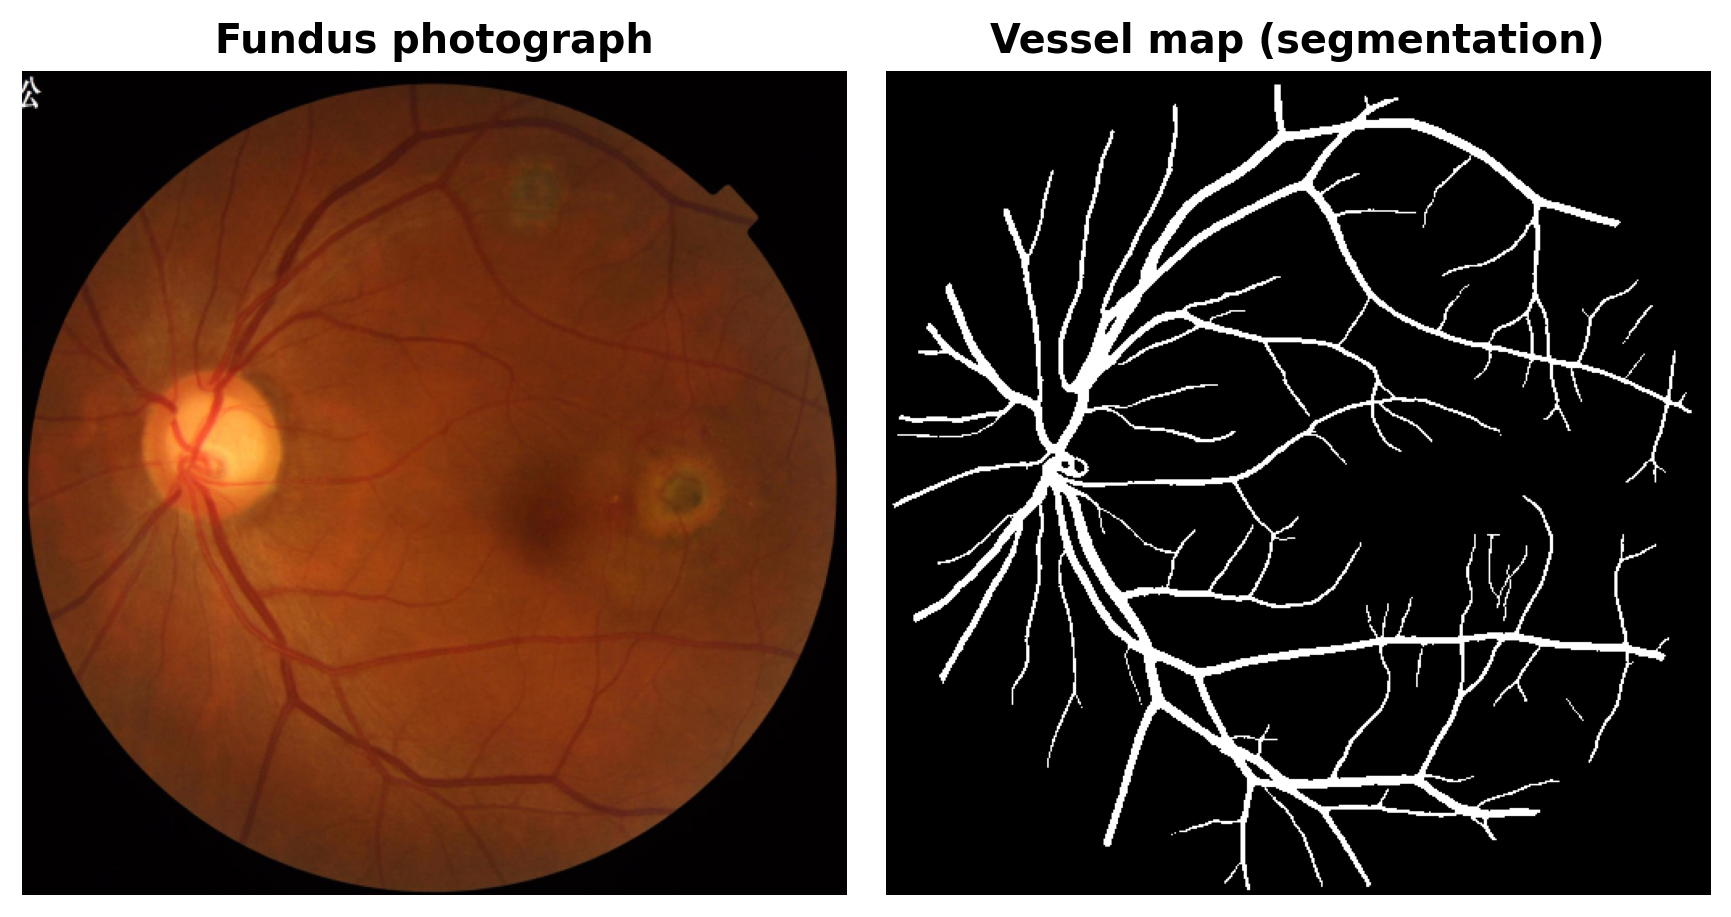
\includegraphics[width=\linewidth]{intro.png}\\[2pt]
      {\scriptsize Input: colour fundus photo. Output: binary vessel map (white = vessel).}
    \end{column}
  \end{columns}
\end{frame}

\begin{frame}{Dataset and objectives}
  \begin{columns}[T]
    \begin{column}{0.52\textwidth}
      \begin{table}
        \caption{The FIVES dataset \cite{jin2022fives} as used in this project.}
        \footnotesize
        \begin{tabular}{@{}ll@{}}
          \toprule
          Images & 800 colour fundus photos, 2048$\times$2048 \\
          Labels & pixel-wise vessel masks (expert consensus) \\
          Groups & AMD, DR, Glaucoma, Normal (200 each) \\
          Train & 480 images (120 per group) \\
          Validation & 120 images (30 per group, stratified) \\
          Test & 200 images (50 per group) -- used once \\
          Working size & 512$\times$512 (baseline), 1024$\times$1024 (ours) \\
          \bottomrule
        \end{tabular}
      \end{table}
    \end{column}
    \begin{column}{0.46\textwidth}
      \textbf{Task:} binary semantic segmentation (vessel vs.\ background).\\[4pt]
      \textbf{Objectives}
      \begin{enumerate}\setlength\itemsep{2pt}
        \item Replicate CAR-UNet \cite{guo2021carunet} on FIVES with a fair protocol.
        \item Modify it to recover thin vessels and keep vessels connected.
        \item Prove every gain with an ablation and significance tests.
      \end{enumerate}
      \textbf{Metrics:} Dice, IoU (main); sensitivity, specificity, accuracy, AUC (as in the paper); clDice (connectivity). Computed inside the retina (FOV), per image, over 3 seeds.
    \end{column}
  \end{columns}
\end{frame}

% =============================================================================== 2. BASE PAPER
\section{Base paper}

\begin{frame}{Base paper: CAR-UNet}
  \begin{block}{Channel Attention Residual U-Net for Retinal Vessel Segmentation}
    C.~Guo, M.~Szemenyei, Y.~Hu, W.~Wang, W.~Zhou, Y.~Yi --- \textbf{IEEE ICASSP 2021} (conference) --- arXiv:2004.03702 \cite{guo2021carunet}
  \end{block}
  \vspace{4pt}
  \begin{columns}[T]
    \begin{column}{0.5\textwidth}
      \textbf{What the paper proposes}
      \begin{itemize}\setlength\itemsep{2pt}
        \item Start from U-Net \cite{ronneberger2015unet}.
        \item Replace every conv block with a \textbf{residual block + channel attention} (CADRB).
        \item Put channel attention (MECA, based on ECA-Net \cite{wang2020eca}) on every \textbf{skip connection}.
        \item Trained with BCE loss and Adam.
      \end{itemize}
    \end{column}
    \begin{column}{0.48\textwidth}
      \begin{table}
        \caption{Results reported in the paper.}
        \scriptsize
        \begin{tabular}{@{}lcccc@{}}
          \toprule
          Dataset & Acc & Sen & Spe & AUC \\
          \midrule
          DRIVE & 0.9699 & 0.8135 & 0.9849 & 0.9852 \\
          CHASE\_DB1 & 0.9751 & 0.8439 & 0.9839 & 0.9898 \\
          STARE & 0.9743 & 0.8445 & 0.9850 & 0.9911 \\
          \bottomrule
        \end{tabular}
      \end{table}
      {\scriptsize The paper does not report Dice or IoU.}
    \end{column}
  \end{columns}
\end{frame}

\begin{frame}{Base architecture and key blocks}
  \begin{columns}[c]
    \begin{column}{0.68\textwidth}
      \centering
      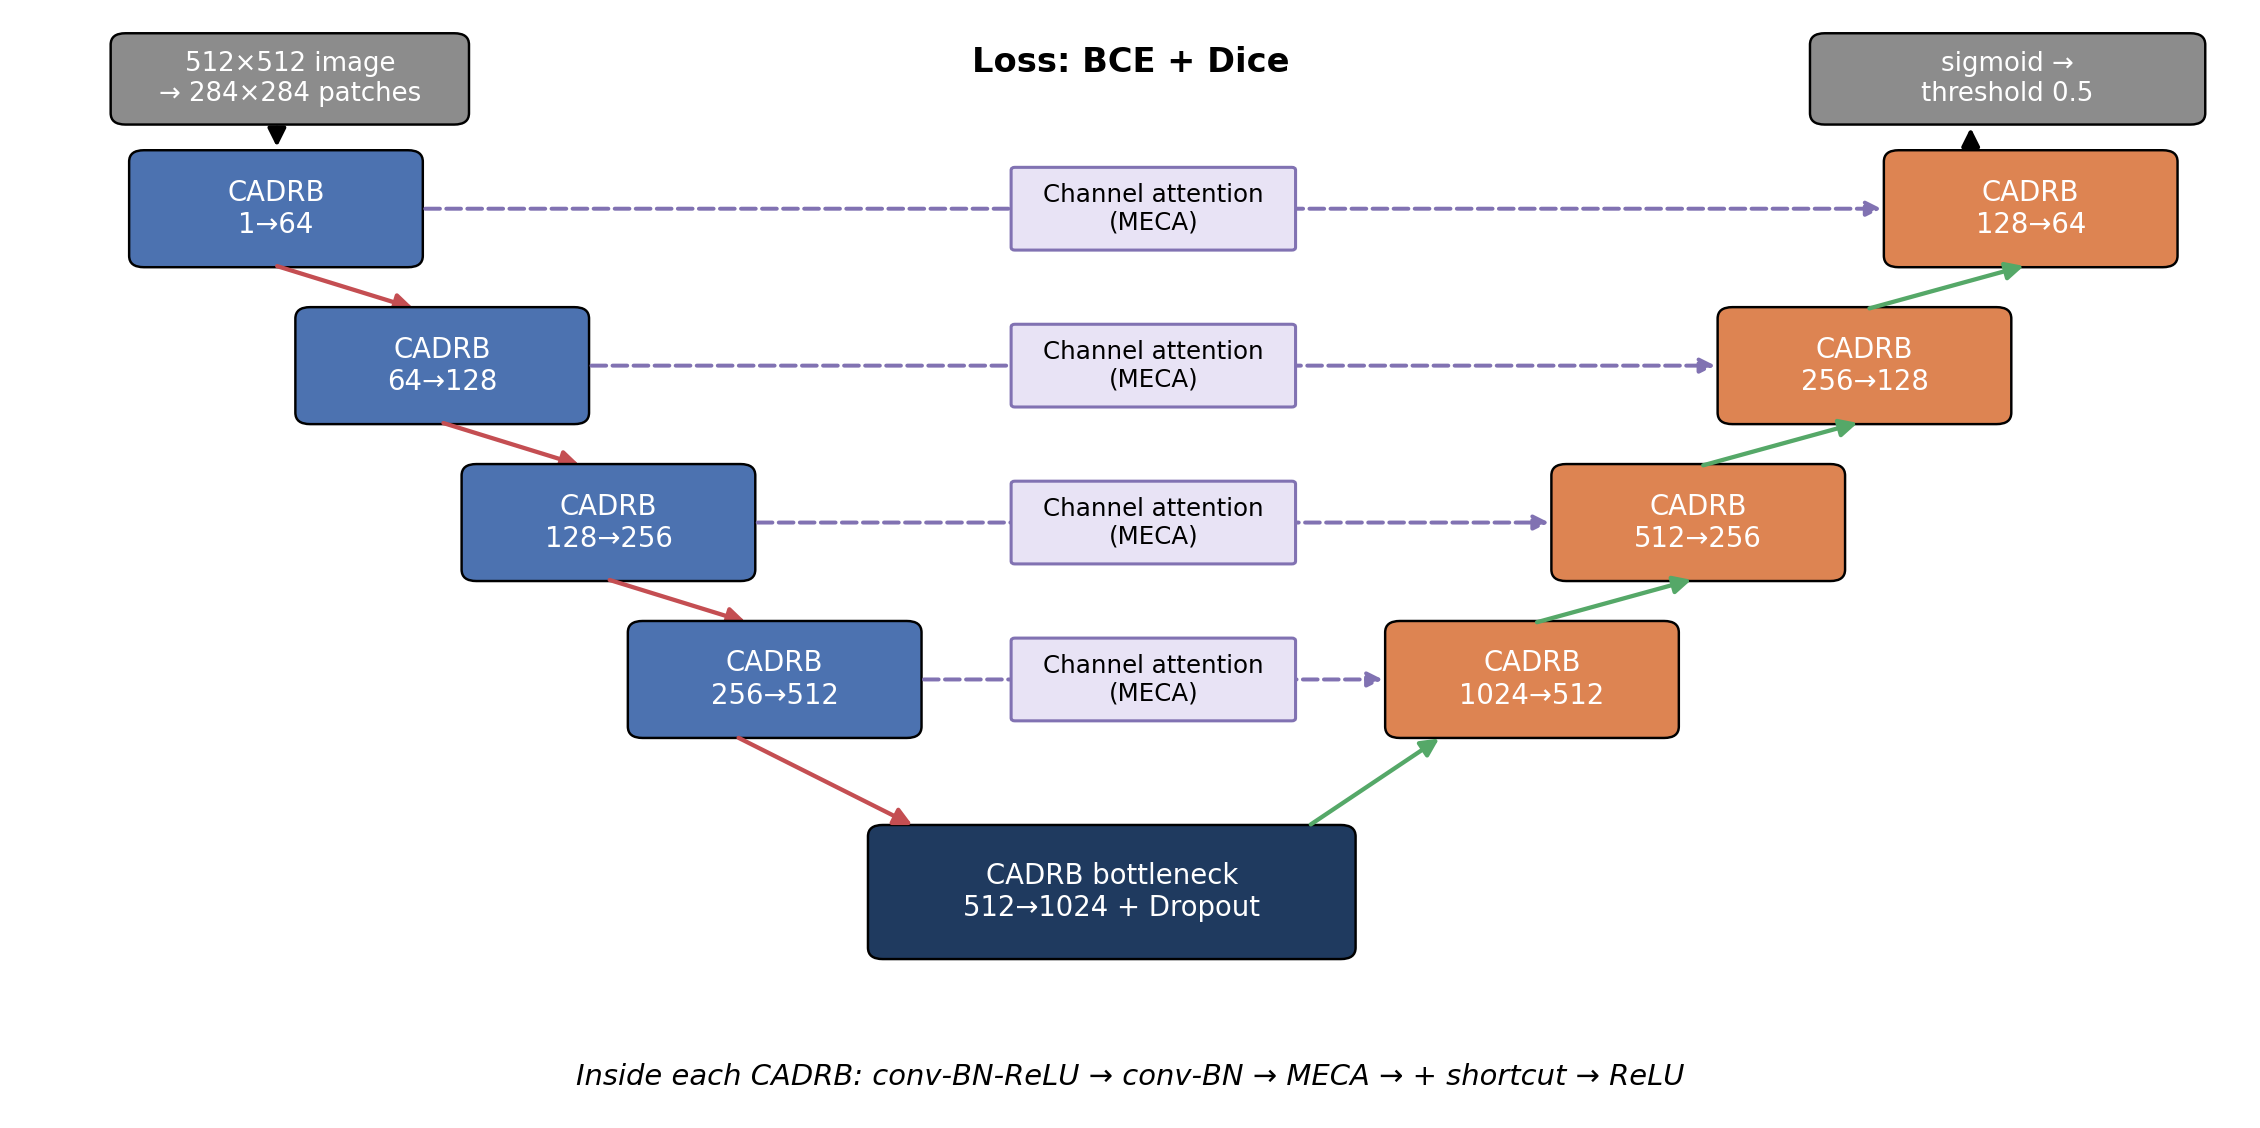
\includegraphics[width=\linewidth]{arch_baseline.png}\\
      {\scriptsize 284$\times$284 input patch $\rightarrow$ 100$\times$100 vessel map (valid convolutions, as in U-Net).}
    \end{column}
    \begin{column}{0.31\textwidth}
      \footnotesize
      \textbf{Encoder / decoder:} encoder finds \emph{what} is in the patch, decoder recovers \emph{where}; skip connections bring back fine detail.\\[5pt]
      \textbf{CADRB:} conv--BN--ReLU $\rightarrow$ conv--BN $\rightarrow$ attention, plus a shortcut. The block only learns a correction, so deep training is stable.\\[5pt]
      \textbf{MECA (channel attention):} one weight per feature channel -- strong detectors are boosted, weak ones damped.\\[5pt]
      \textbf{Skip attention:} encoder features are re-weighted before they reach the decoder.
    \end{column}
  \end{columns}
\end{frame}

\begin{frame}{Replicated vs.\ reported results}
  \begin{table}
    \caption{Paper results (as reported) next to our replication on FIVES. Ours: 200 test images, mean $\pm$ std over 3 seeds.}
    \scriptsize
    \begin{tabular}{@{}llcccccc@{}}
      \toprule
      Model & Dataset & \textbf{Dice} & \textbf{IoU} & Acc & Sen & Spe & AUC \\
      \midrule
      CAR-UNet -- paper (reported) & DRIVE & n/r & n/r & 0.9699 & 0.8135 & 0.9849 & 0.9852 \\
      CAR-UNet -- paper (reported) & CHASE\_DB1 & n/r & n/r & 0.9751 & 0.8439 & 0.9839 & 0.9898 \\
      \rowcolor{navy!8}
      \textbf{CAR-UNet -- our replication} & \textbf{FIVES} & \textbf{0.8382 $\pm$ 0.0031} & \textbf{0.7295 $\pm$ 0.0043} & 0.9728 & 0.8310 & 0.9855 & 0.9860 \\
      U-Net -- our reference & FIVES & 0.8344 $\pm$ 0.0034 & 0.7246 $\pm$ 0.0050 & 0.9723 & 0.8247 & 0.9852 & 0.9847 \\
      \bottomrule
    \end{tabular}
  \end{table}
  \begin{itemize}\setlength\itemsep{3pt}\small
    \item Our accuracy, specificity and AUC land in the same range as the paper; sensitivity is in between its DRIVE and CHASE values.
    \item Numbers are not one-to-one: the paper used small single-source sets (20--40 images), we use the 800 multi-disease FIVES images required for this project.
    \item CAR-UNet beats U-Net on \textbf{154 / 200} test images (paired Wilcoxon, $p = 2\times10^{-14}$) -- the replication reproduces the paper's claim.
    \item Honest difference: we kept U-Net's valid-convolution geometry, 64 base filters and Dropout (paper: 16 filters, DropBlock).
  \end{itemize}
\end{frame}

\begin{frame}{Replicated model: sample predictions}
  \begin{columns}[c]
    \begin{column}{0.46\textwidth}
      \centering
      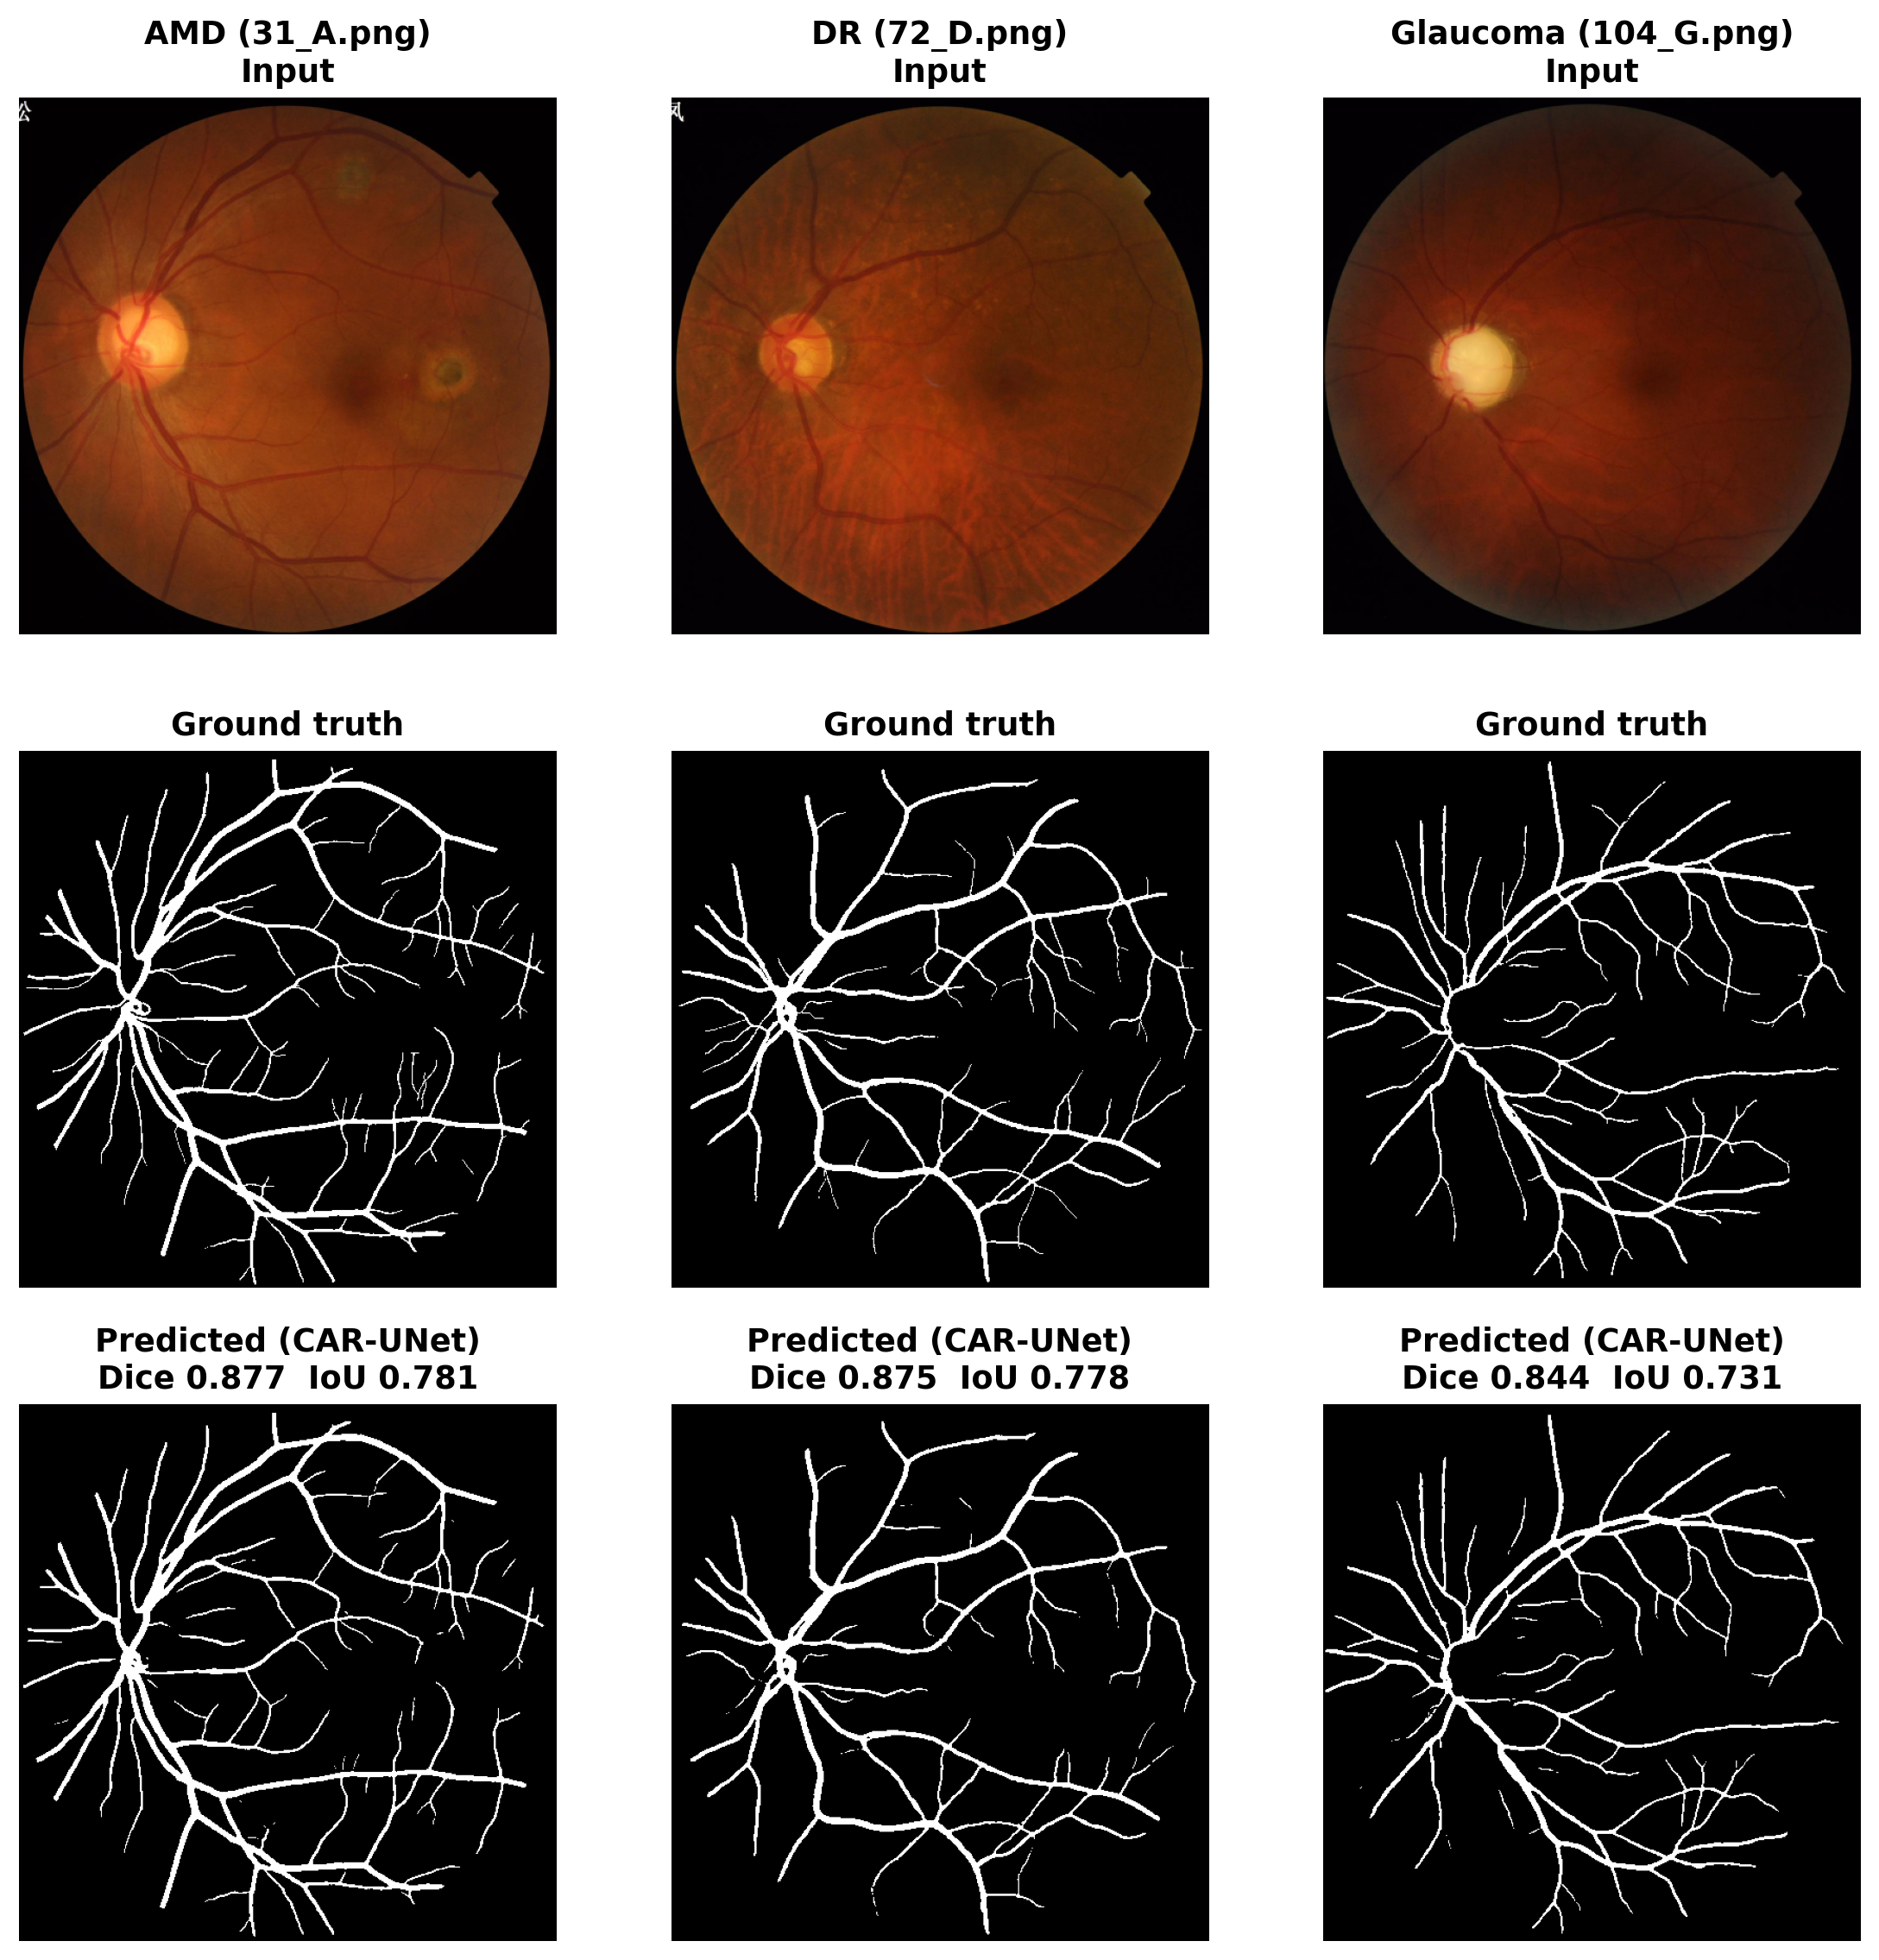
\includegraphics[height=0.82\textheight]{replicated_samples.png}
    \end{column}
    \begin{column}{0.52\textwidth}
      \begin{itemize}\setlength\itemsep{6pt}
        \item Three test images from three disease groups (median-Dice cases, not hand-picked).
        \item Rows: \textbf{input}, \textbf{expert ground truth}, \textbf{our predicted mask}.
        \item Thick vessels are traced almost perfectly.
        \item What goes wrong: \textbf{thin capillaries} at vessel ends are missed or broken into pieces -- this is what our modification targets.
      \end{itemize}
    \end{column}
  \end{columns}
\end{frame}

% =============================================================================== 3. IMPLEMENTATION
\section{Implementation}

\begin{frame}[fragile]{Code structure and training settings}
  \begin{columns}[T]
    \begin{column}{0.5\textwidth}
      \textbf{Code} (PyTorch) -- \href{https://github.com/Abhishek-karthik/Retinal-Vessel-Segmentation-CAR-UNet}{\textcolor{blue}{GitHub repository}}
\begin{semiverbatim}\footnotesize
src/
 preprocessing_fives.py  \textcolor{gray}{green, CLAHE, bilateral}
 data_loader_fives.py    \textcolor{gray}{split, patches, augment}
 car_unet.py             \textcolor{gray}{CAR-UNet (+ dual attn)}
 losses.py               \textcolor{gray}{BCE + Dice (+ clDice)}
 metrics.py              \textcolor{gray}{FOV metrics, clDice}
 utils.py                \textcolor{gray}{overlap-tile inference}
scripts/
 train_fives.py          \textcolor{gray}{training loop + test}
 evaluate_post.py        \textcolor{gray}{threshold / TTA}
 summarize_*.py          \textcolor{gray}{tables, Wilcoxon tests}
\end{semiverbatim}
      \footnotesize Pipeline: load + preprocess $\rightarrow$ random 284$\times$284 patches $\rightarrow$ model $\rightarrow$ loss $\rightarrow$ full-image prediction (overlap-tile) $\rightarrow$ metrics.
    \end{column}
    \begin{column}{0.48\textwidth}
      \begin{table}
        \caption{Training settings (identical for every model).}
        \footnotesize
        \begin{tabular}{@{}ll@{}}
          \toprule
          Framework & PyTorch 2.6, CUDA 12.4 \\
          Optimizer & Adam, weight decay $10^{-5}$ \\
          Learning rate & $10^{-3}$, cosine decay \\
          Batch size & 8 patches (284$\times$284) \\
          Patches & 6 fresh per image per epoch \\
          Epochs & 30 (best val-Dice checkpoint) \\
          Loss & 0.5 BCE + 0.5 Dice \\
          Augmentation & flips, 90$^\circ$ rotations, elastic \\
          Seeds & 3 per model \\
          Hardware & RTX 4050 laptop GPU (6 GB) \\
          Time & $\approx$91 min per run (CAR-UNet) \\
          \bottomrule
        \end{tabular}
      \end{table}
    \end{column}
  \end{columns}
\end{frame}

\begin{frame}{Training logs and curves}
  \begin{columns}[c]
    \begin{column}{0.53\textwidth}
      \centering
      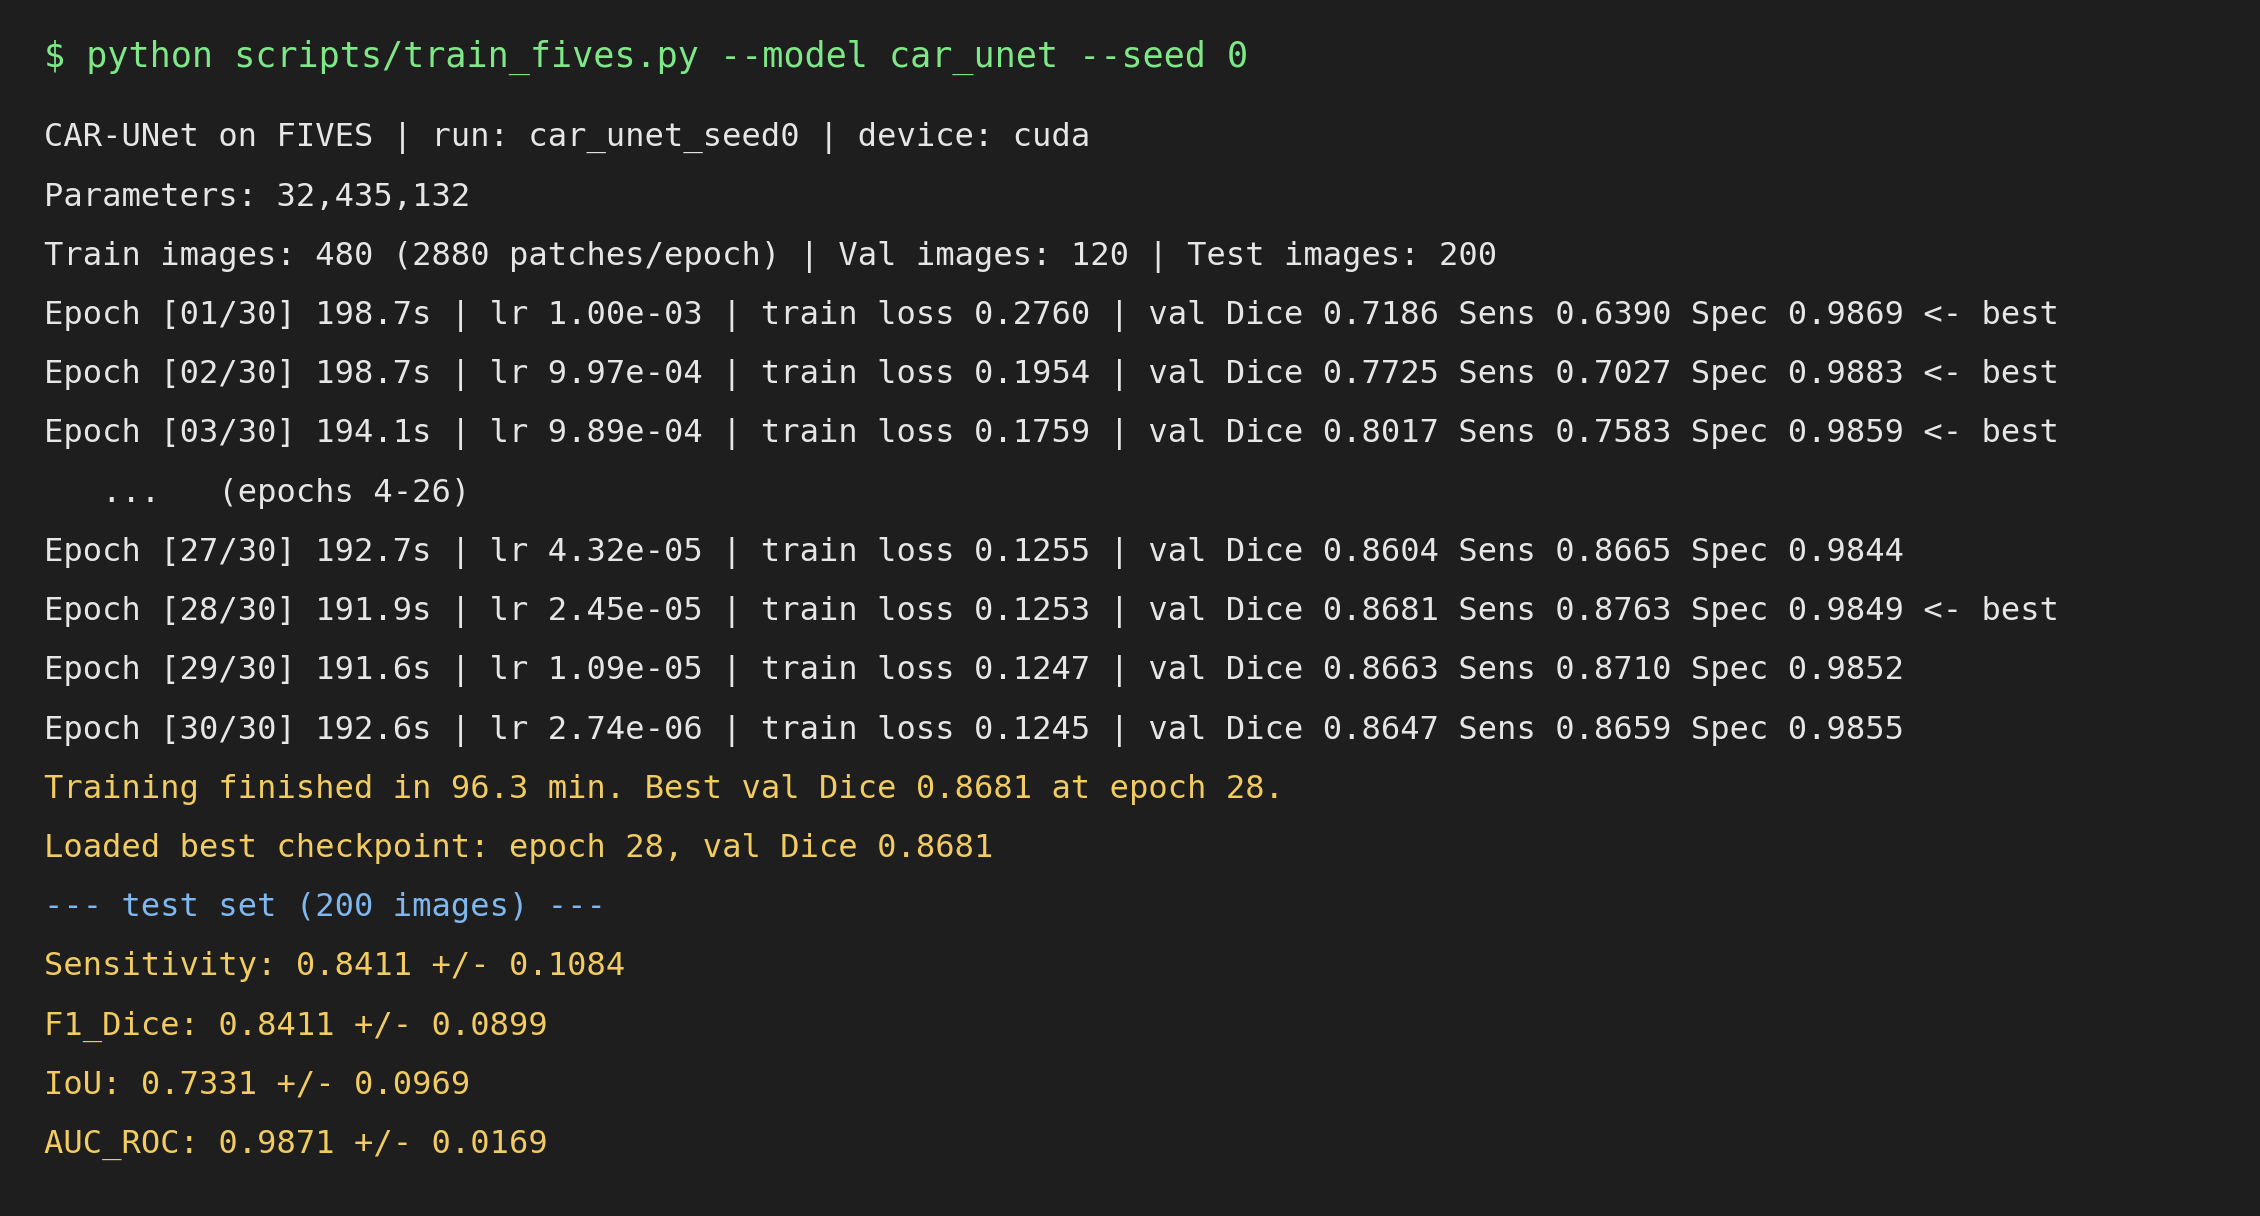
\includegraphics[width=\linewidth]{training_log.png}\\
      {\scriptsize Real training log of the replicated CAR-UNet (seed 0).}
      \begin{itemize}\setlength\itemsep{1pt}\footnotesize
        \item Loss falls smoothly; no sign of overfitting.
        \item Validation Dice levels off near 0.86 by epoch $\sim$25, so 30 epochs is enough.
        \item The best epoch is picked on validation images, never on test images.
      \end{itemize}
    \end{column}
    \begin{column}{0.46\textwidth}
      \centering
      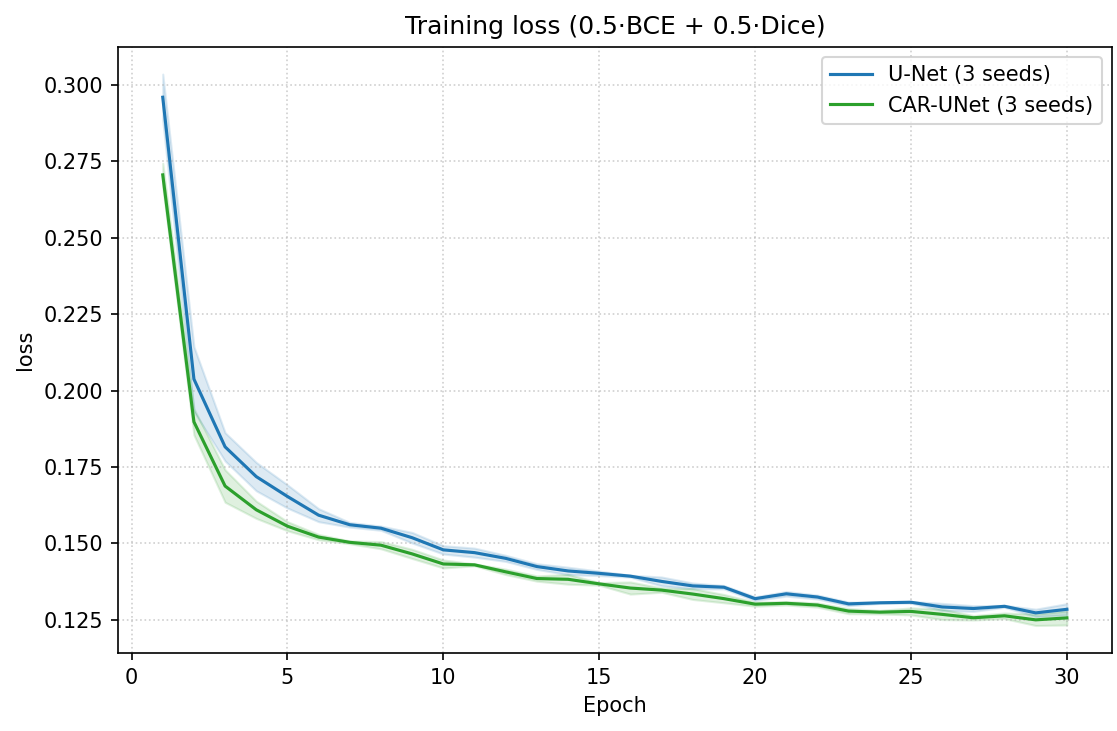
\includegraphics[height=0.35\textheight]{curve_loss.png}\\[2pt]
      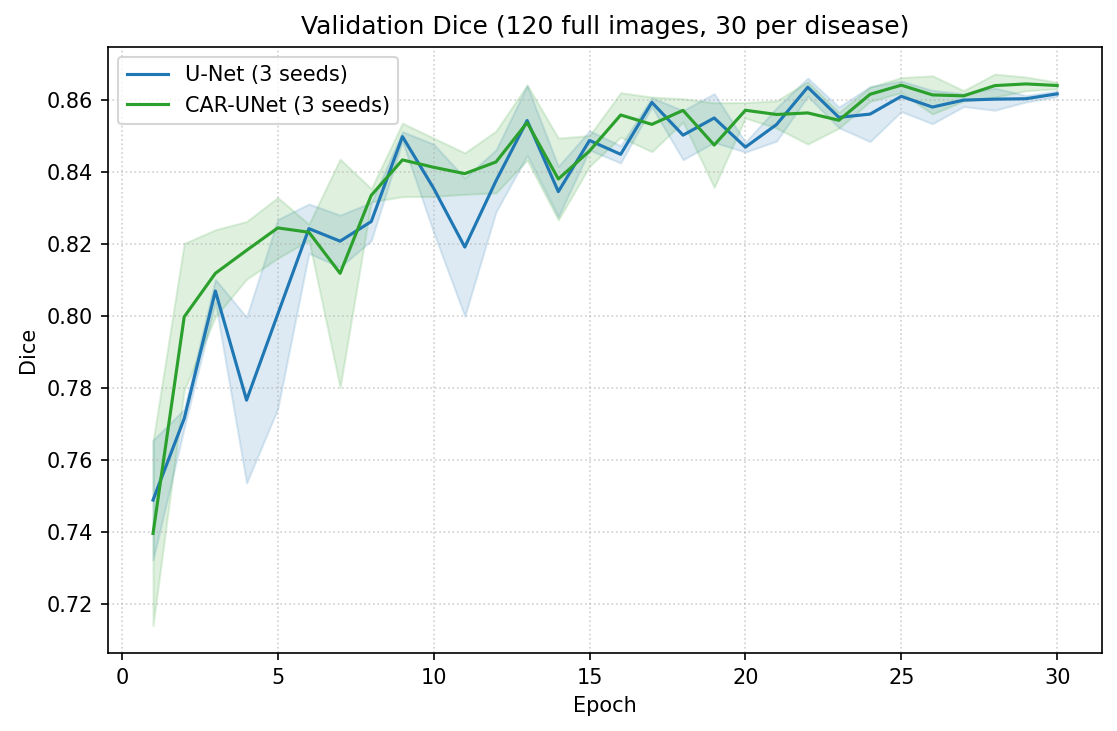
\includegraphics[height=0.35\textheight]{curve_valdice.png}\\
      {\scriptsize Loss and validation Dice, mean $\pm$ std over 3 seeds (U-Net vs.\ CAR-UNet).}
    \end{column}
  \end{columns}
\end{frame}

% =============================================================================== 4. MODIFICATION
\section{Modification}

\begin{frame}{What we changed -- and why}
  \begin{table}
    \caption{Each modification targets one weakness of the base paper. Data split, seeds, optimizer, epochs and augmentation stay identical to the baseline.}
    \scriptsize
    \begin{tabular}{@{}p{0.30\textwidth}p{0.49\textwidth}p{0.15\textwidth}@{}}
      \toprule
      \textbf{Weakness of CAR-UNet} & \textbf{Our modification} & \textbf{Type} \\
      \midrule
      Channel attention says \emph{which} features matter, not \emph{where} the vessels are &
      \textbf{1. Dual attention:} channel (avg + max pooling) + spatial attention (CBAM \cite{woo2018cbam}) in all 13 attention modules & attention module \\
      BCE counts pixels, so a broken thin vessel costs almost nothing &
      \textbf{2. clDice loss} \cite{shit2021cldice}: compares vessel skeletons, rewards connected vessels & loss function \\
      At 512$\times$512 the finest capillaries are erased &
      \textbf{3. 1024$\times$1024 working resolution}, scored on the same 512 ground truth & input resolution \\
      Fixed 0.5 decision threshold &
      \textbf{4. Threshold chosen on validation} (0.44--0.48); flip TTA tested too & prediction \\
      \bottomrule
    \end{tabular}
  \end{table}
  \vspace{1pt}
  \begin{columns}[T]
    \begin{column}{0.32\textwidth}
      \centering
      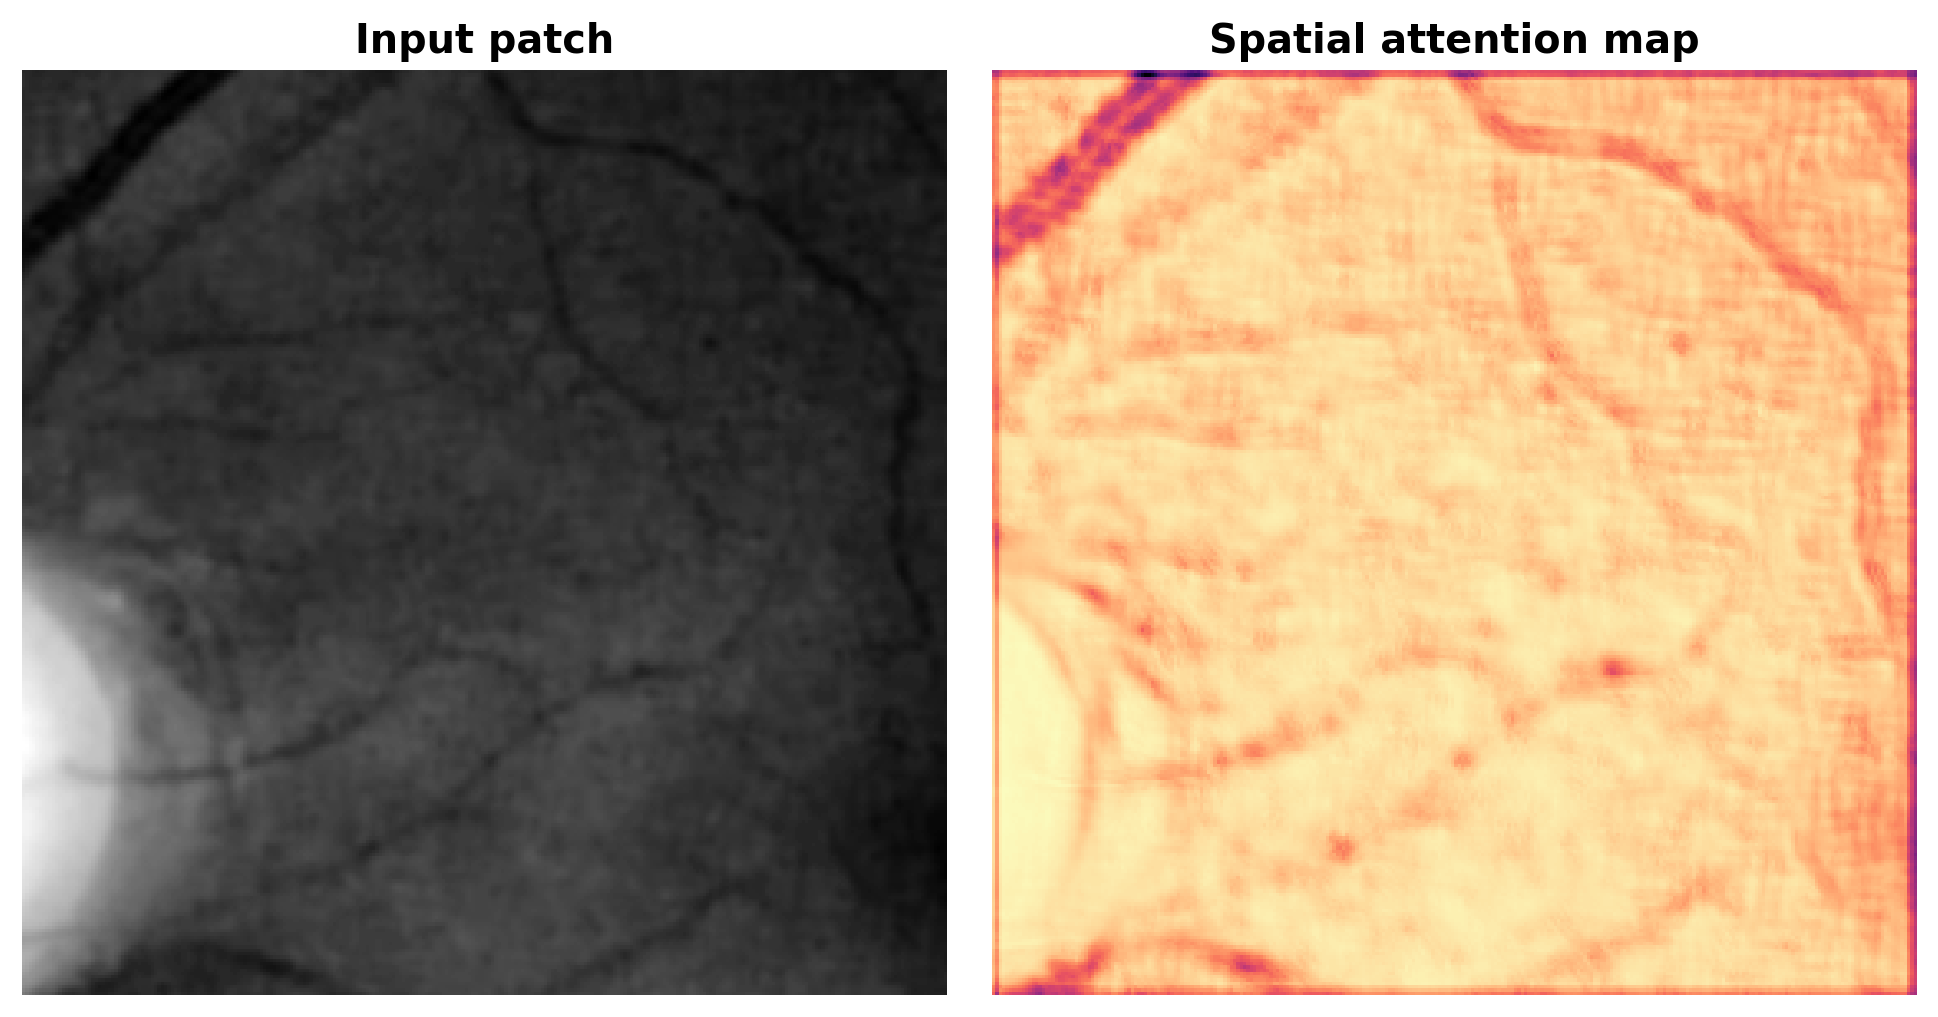
\includegraphics[width=0.80\linewidth]{ev_attention.png}\\
      \tiny \textbf{Dual attention:} the spatial attention map traces the vessel tree -- the network knows \emph{where} vessels are.
    \end{column}
    \begin{column}{0.32\textwidth}
      \centering
      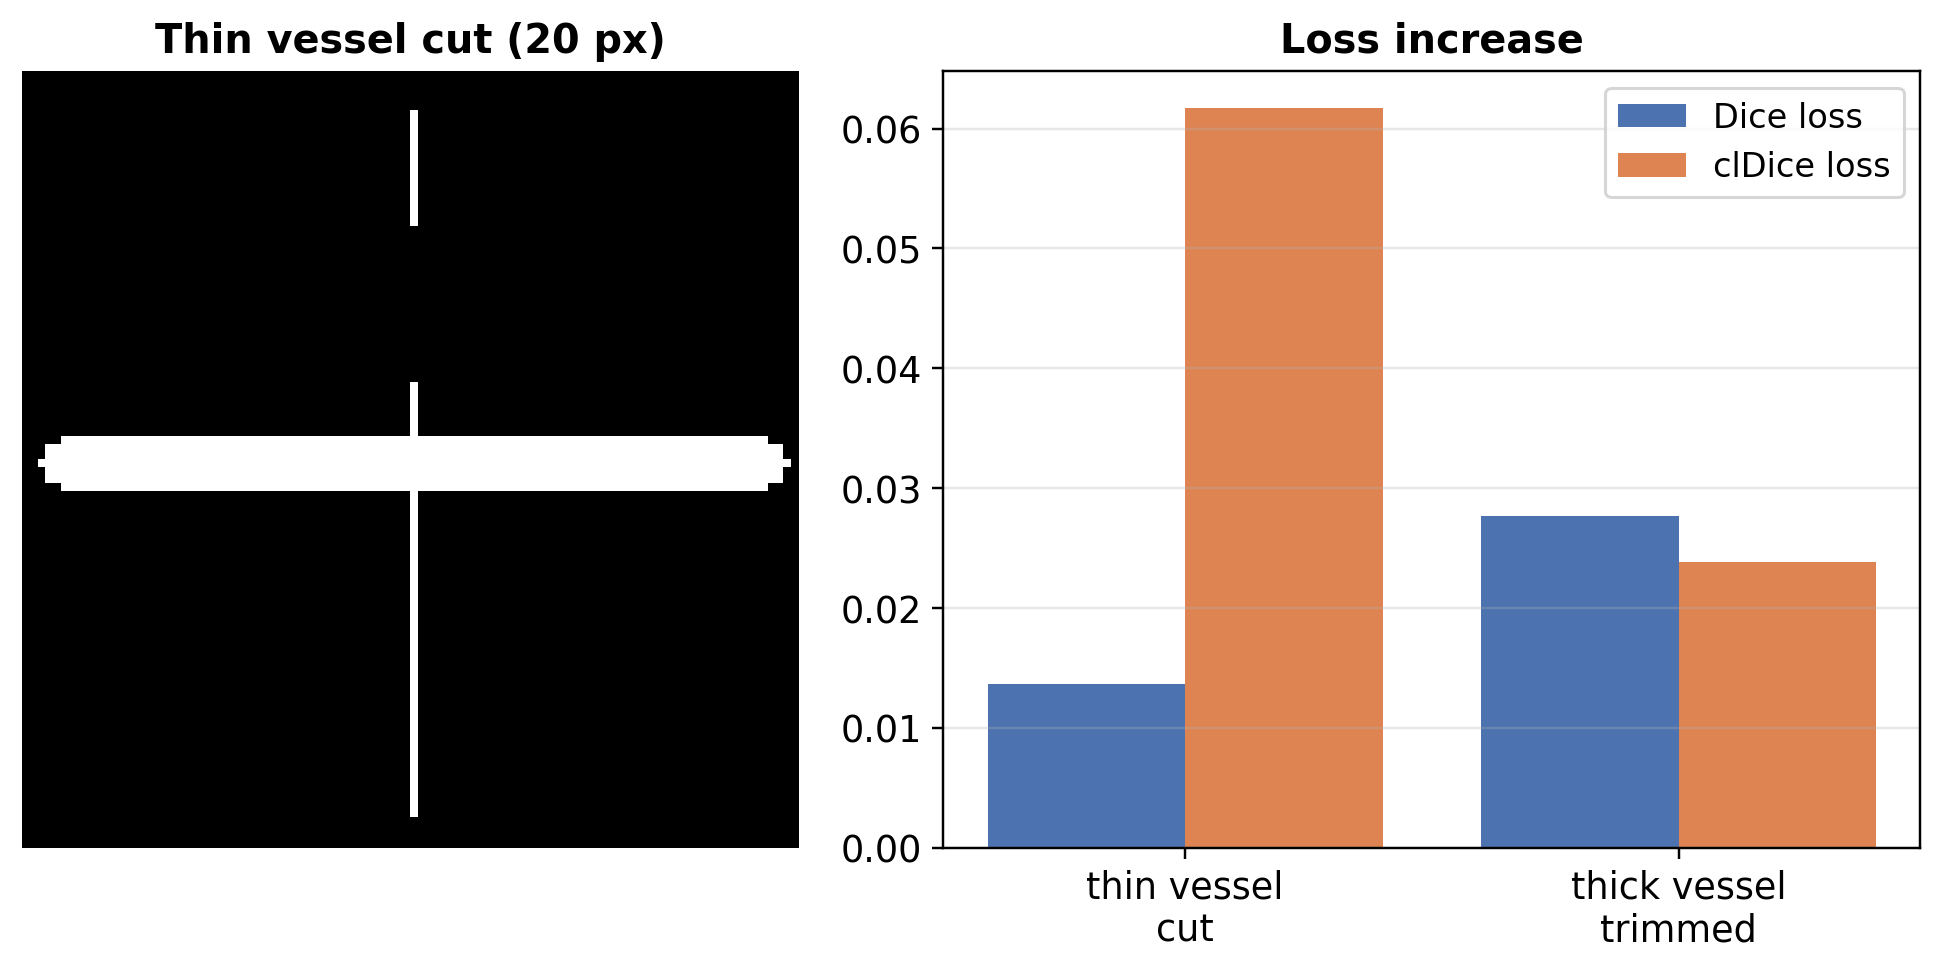
\includegraphics[width=0.80\linewidth]{ev_cldice.png}\\
      \tiny \textbf{clDice:} a cut thin vessel raises the clDice loss \textbf{4.5$\times$} more than the Dice loss.
    \end{column}
    \begin{column}{0.32\textwidth}
      \centering
      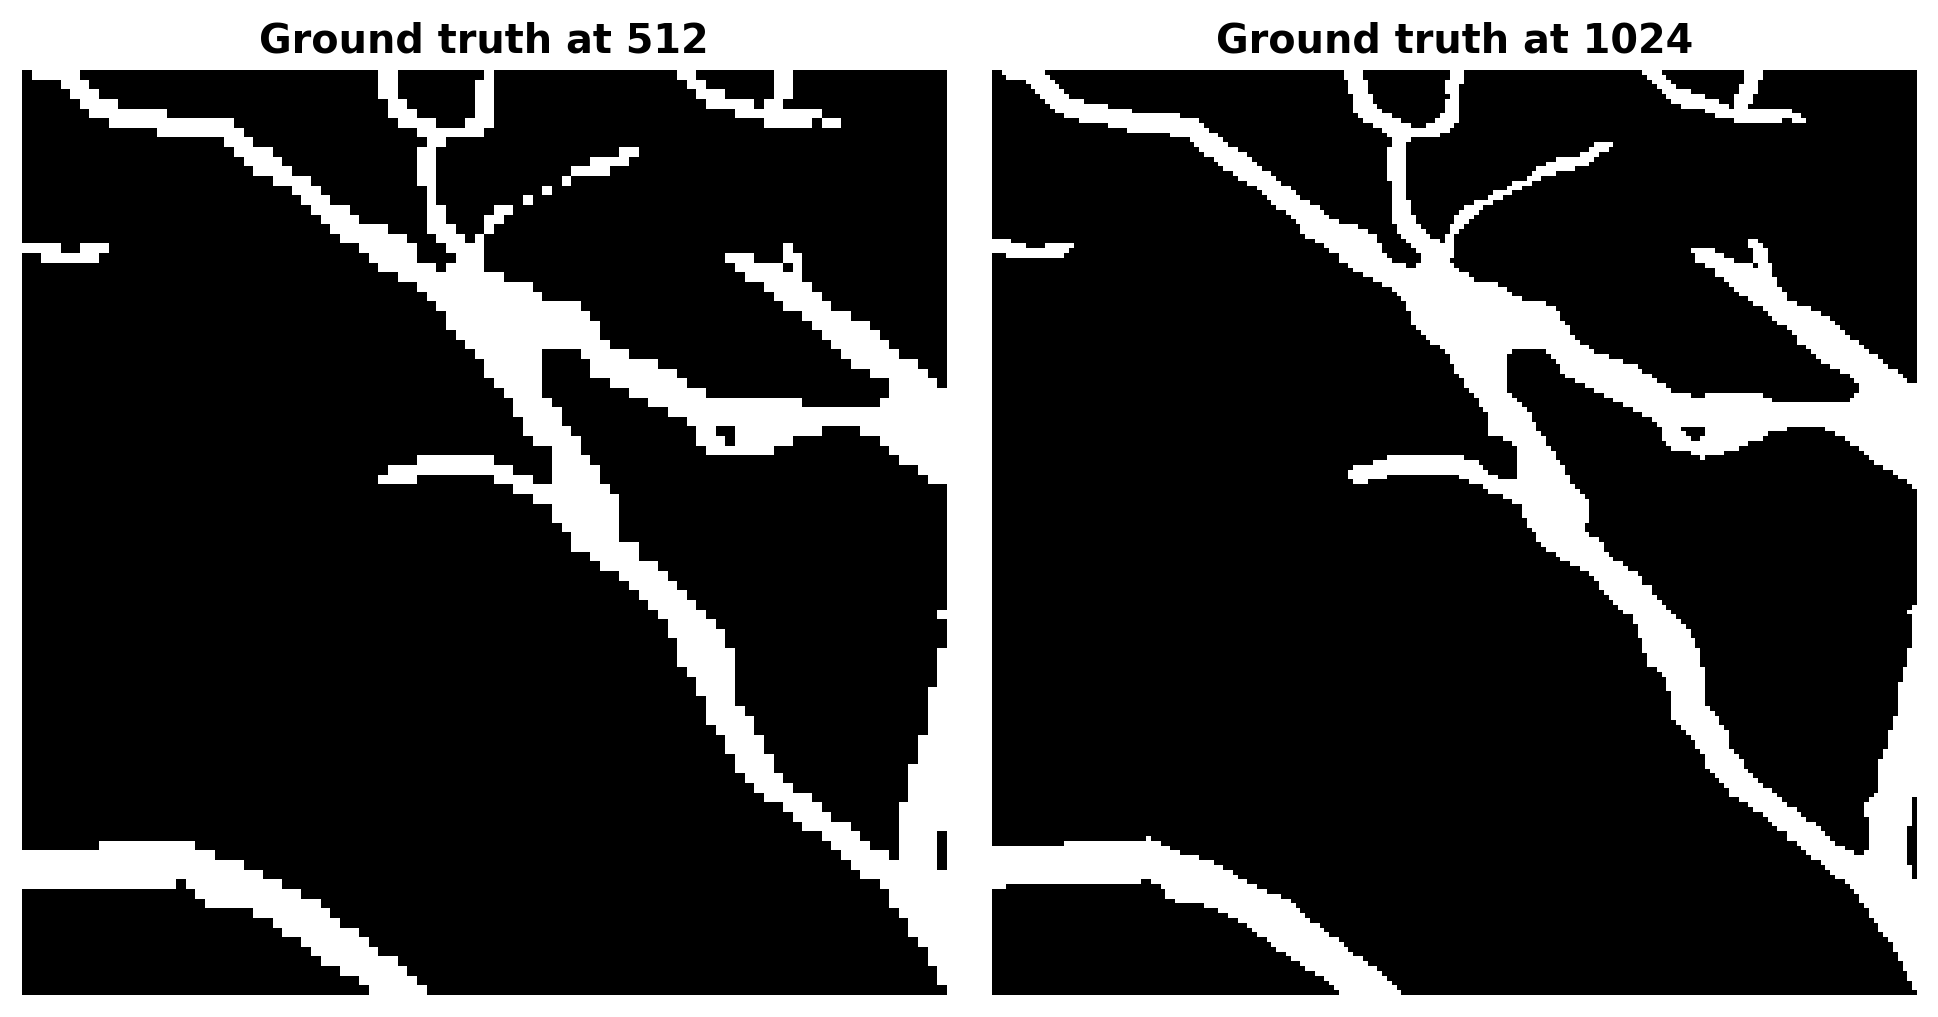
\includegraphics[width=0.80\linewidth]{ev_resolution.png}\\
      \tiny \textbf{1024:} thin vessels broken at 512 are continuous at 1024 -- the model can only learn what it sees.
    \end{column}
  \end{columns}
\end{frame}

\begin{frame}{Modified architecture}
  \begin{columns}[c]
    \begin{column}{0.68\textwidth}
      \centering
      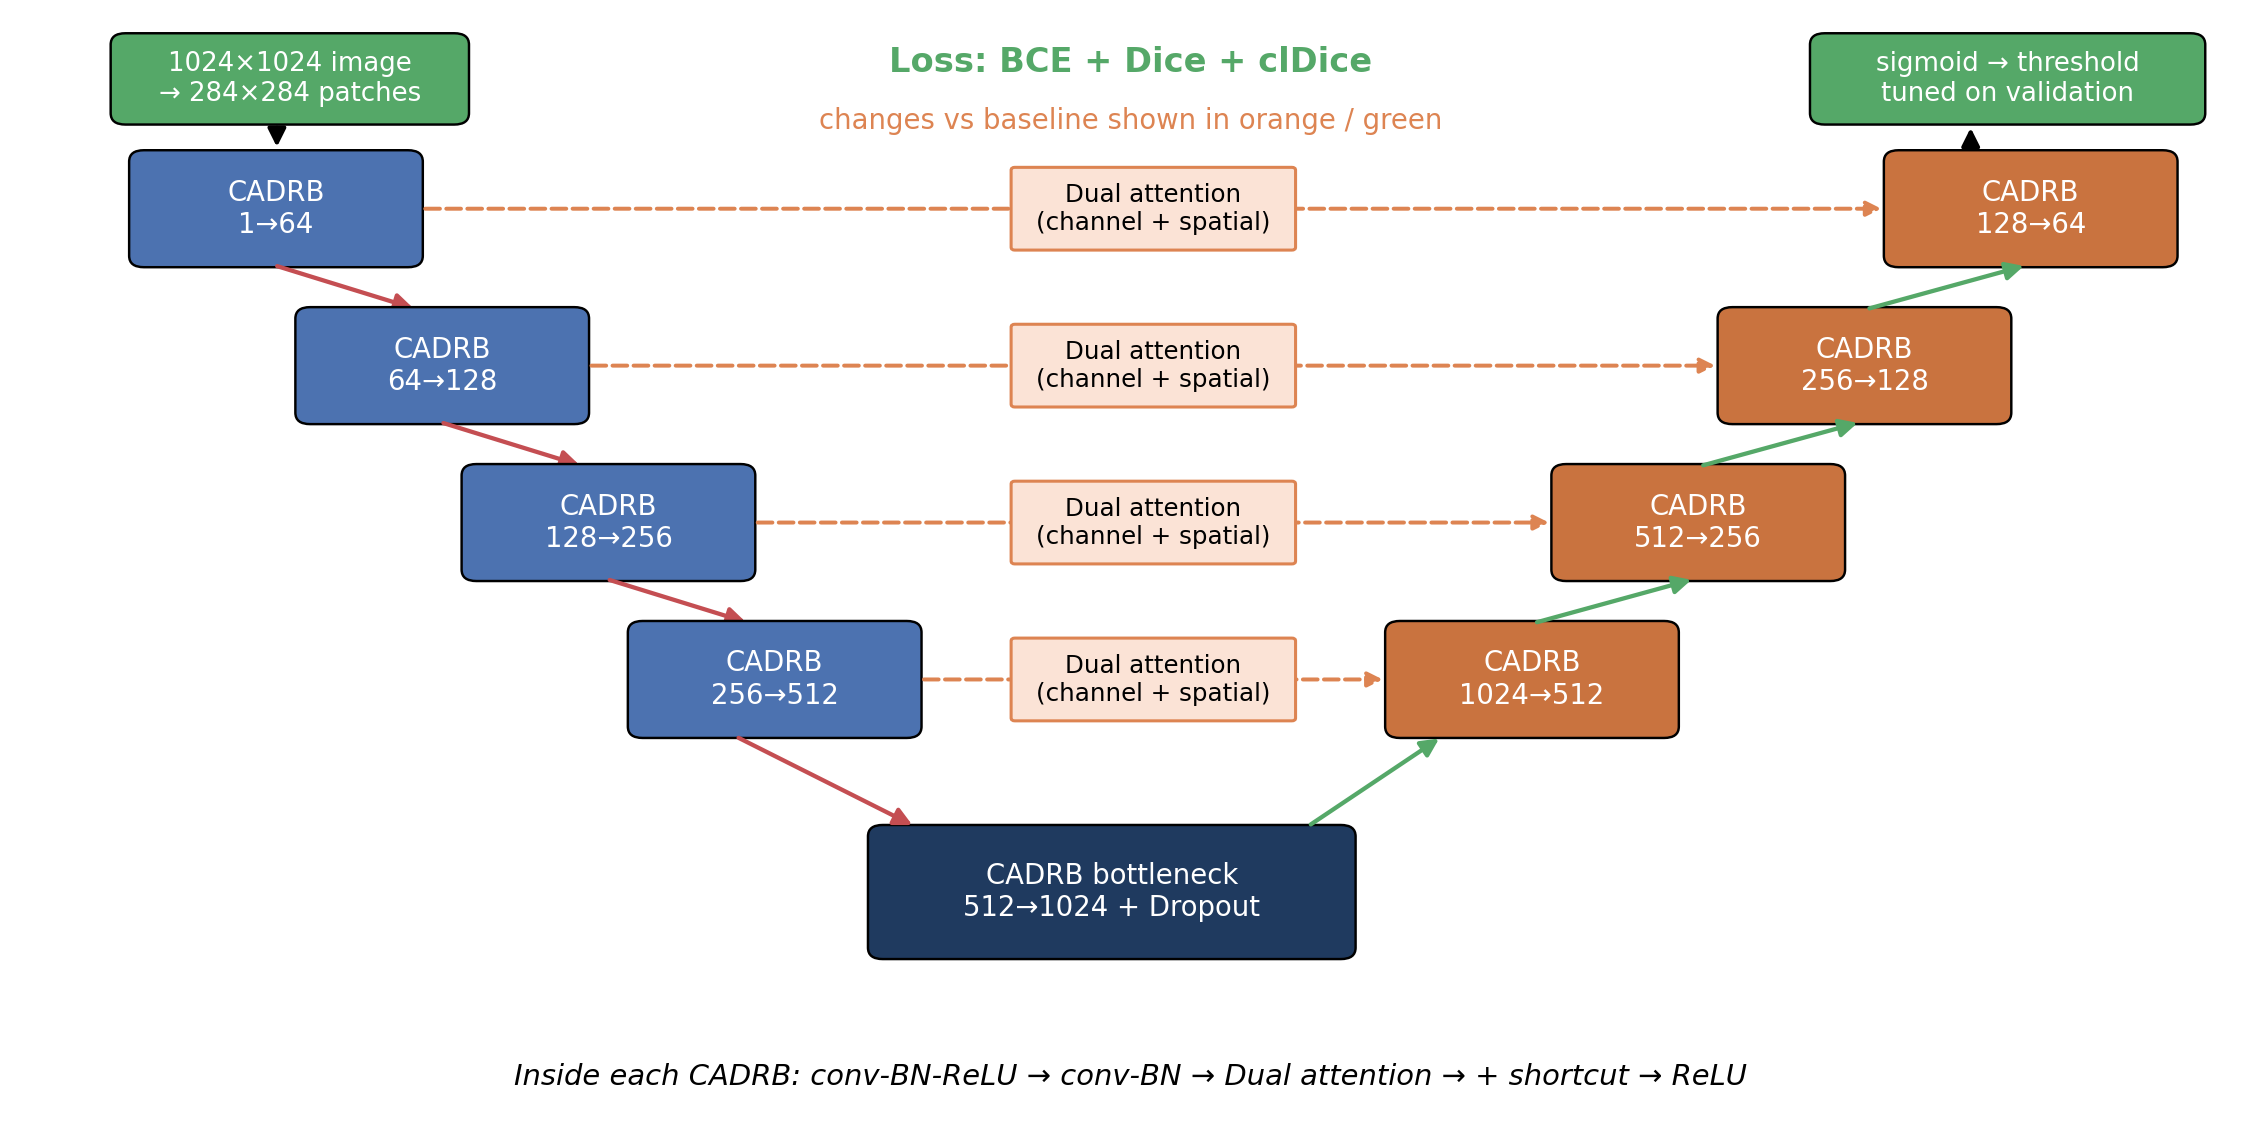
\includegraphics[width=\linewidth]{arch_modified.png}\\
      {\scriptsize Changes vs.\ the baseline in orange/green: dual attention everywhere, 1024 input, clDice loss, tuned threshold.}
    \end{column}
    \begin{column}{0.31\textwidth}
      \centering
      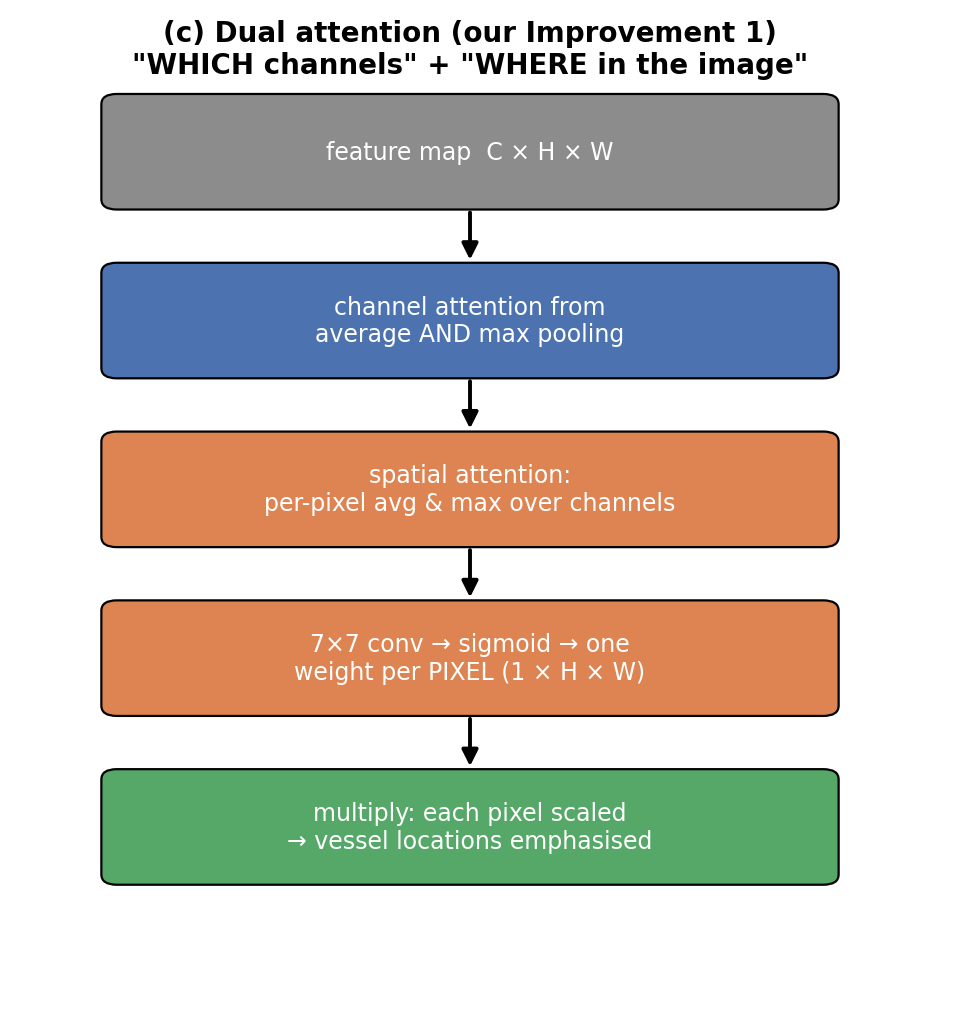
\includegraphics[width=\linewidth]{dual_attention_block.png}\\
      {\scriptsize Dual attention: per-channel weights \emph{and} one weight per pixel. Only \textbf{+1,274 parameters}.}
    \end{column}
  \end{columns}
\end{frame}

\begin{frame}{Comparison: baseline vs.\ modified model}
  \begin{columns}[c]
    \begin{column}{0.57\textwidth}
      \begin{table}
        \caption{Same data split, seeds and settings. 200 test images, mean over 3 seeds; $p$ = paired Wilcoxon test.}
        \scriptsize
        \begin{tabular}{@{}lcccc@{}}
          \toprule
          Metric & Baseline & Modified & Change & $p$ \\
          \midrule
          \textbf{Dice} & 0.8382 $\pm$ .0031 & \textbf{0.8436 $\pm$ .0027} & \up{+0.54} & $5\times10^{-10}$ \\
          \textbf{IoU} & 0.7295 $\pm$ .0043 & \textbf{0.7379 $\pm$ .0039} & \up{+0.83} & $2\times10^{-10}$ \\
          Sensitivity & 0.8310 & \textbf{0.8465} & \up{+1.55} & $7\times10^{-19}$ \\
          Specificity & 0.9855 & 0.9846 & \down{$-$0.09} & $6\times10^{-15}$ \\
          Accuracy & 0.9728 & \textbf{0.9737} & \up{+0.09} & $2\times10^{-8}$ \\
          AUC-ROC & 0.9860 & \textbf{0.9878} & \up{+0.17} & $1\times10^{-21}$ \\
          clDice & 0.8626 $\pm$ .0057 & \textbf{0.8751 $\pm$ .0005} & \up{+1.25} & $5\times10^{-25}$ \\
          \bottomrule
        \end{tabular}
      \end{table}
      {\scriptsize Change in percentage points. Dice better on 140/200 images, connectivity on 175/200; better in all 3 seeds.}
    \end{column}
    \begin{column}{0.42\textwidth}
      \centering
      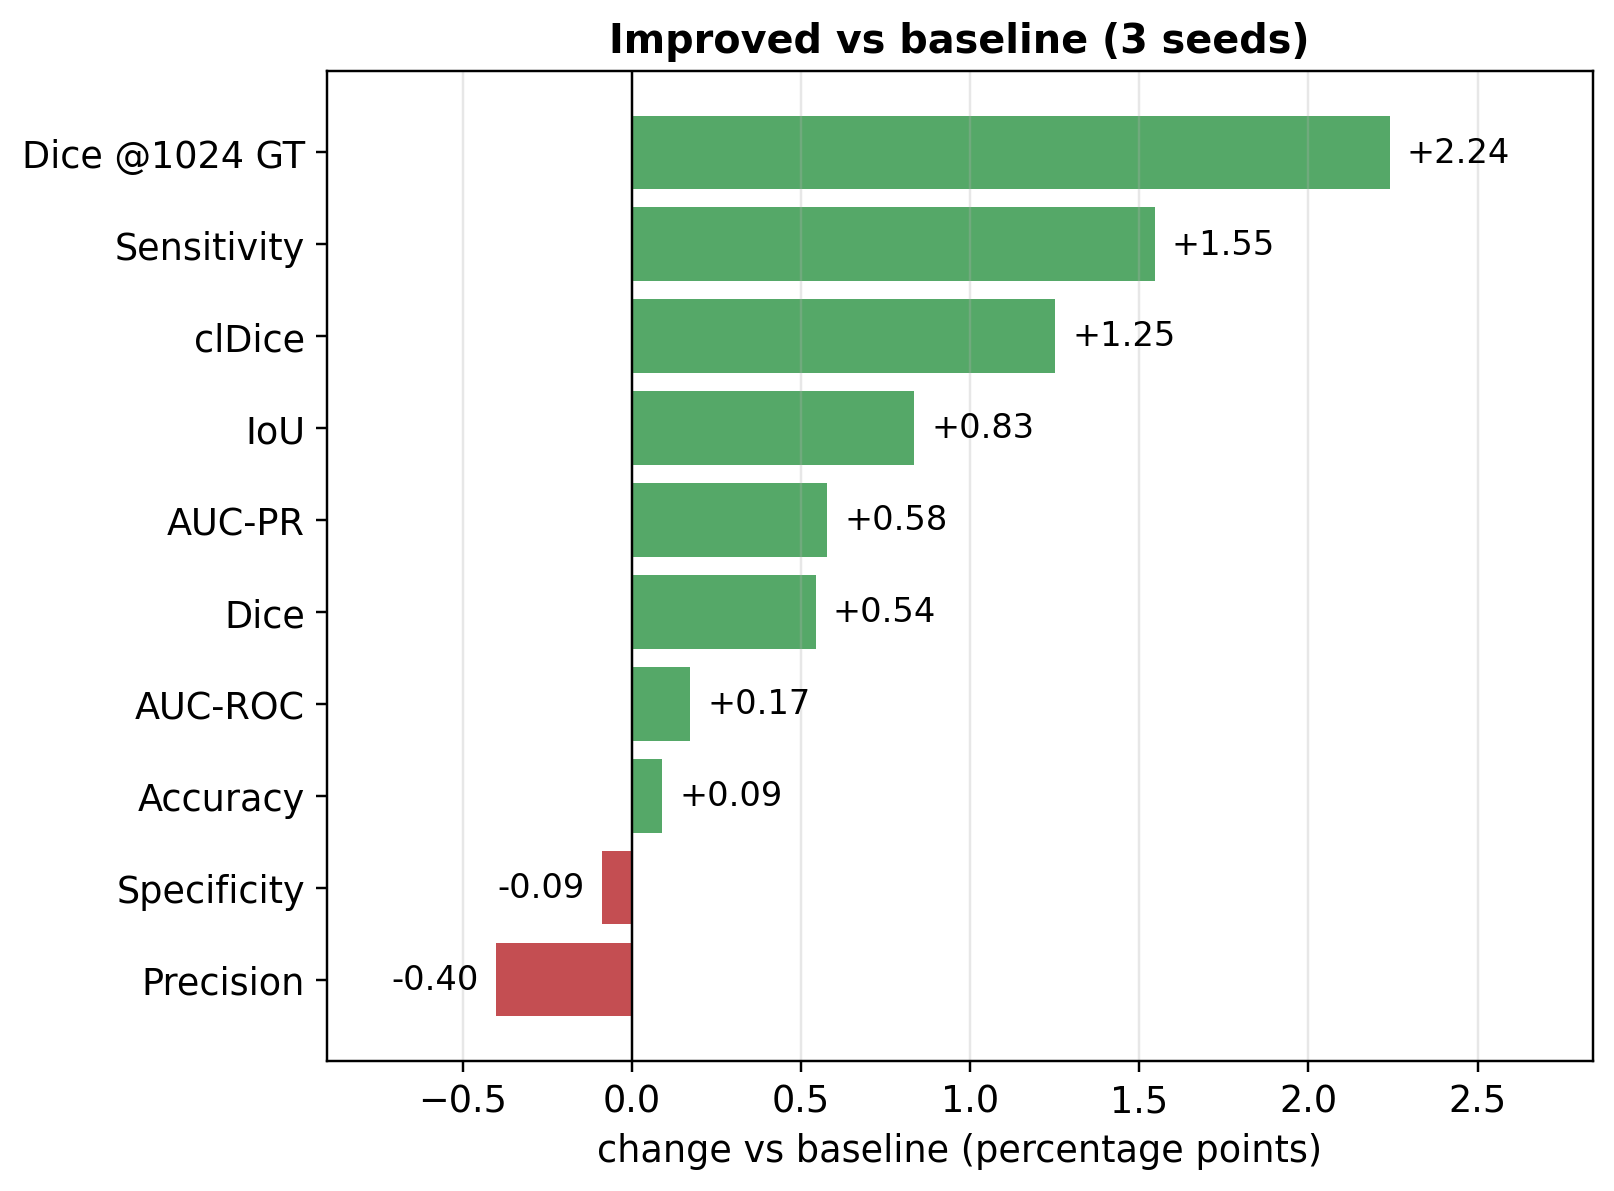
\includegraphics[width=\linewidth]{change_per_metric.png}
    \end{column}
  \end{columns}
\end{frame}

\begin{frame}{Ablation: what each component contributes}
  \begin{table}
    \caption{Adding one modification at a time (3 seeds each, mean $\pm$ std).}
    \scriptsize
    \begin{tabular}{@{}lccccc@{}}
      \toprule
      Step & Dice & IoU & Sensitivity & Precision & clDice \\
      \midrule
      Baseline CAR-UNet & 0.8382 $\pm$ .0031 & 0.7295 & 0.8310 & 0.8557 & 0.8626 \\
      + Dual attention & 0.8408 $\pm$ .0021 & 0.7339 & 0.8308 & \textbf{0.8620} & 0.8631 \\
      + clDice loss & 0.8382 $\pm$ .0050 & 0.7293 & 0.8432 & 0.8430 & 0.8718 \\
      + 1024 resolution & 0.8421 $\pm$ .0028 & 0.7359 & 0.8326 & \textbf{0.8632} & 0.8742 \\
      \rowcolor{accent!15}
      + Tuned threshold (final) & \textbf{0.8436 $\pm$ .0027} & \textbf{0.7379} & \textbf{0.8465} & 0.8516 & \textbf{0.8751} \\
      \bottomrule
    \end{tabular}
  \end{table}
  \vspace{-4pt}
  \begin{columns}[c]
    \begin{column}{0.6\textwidth}
      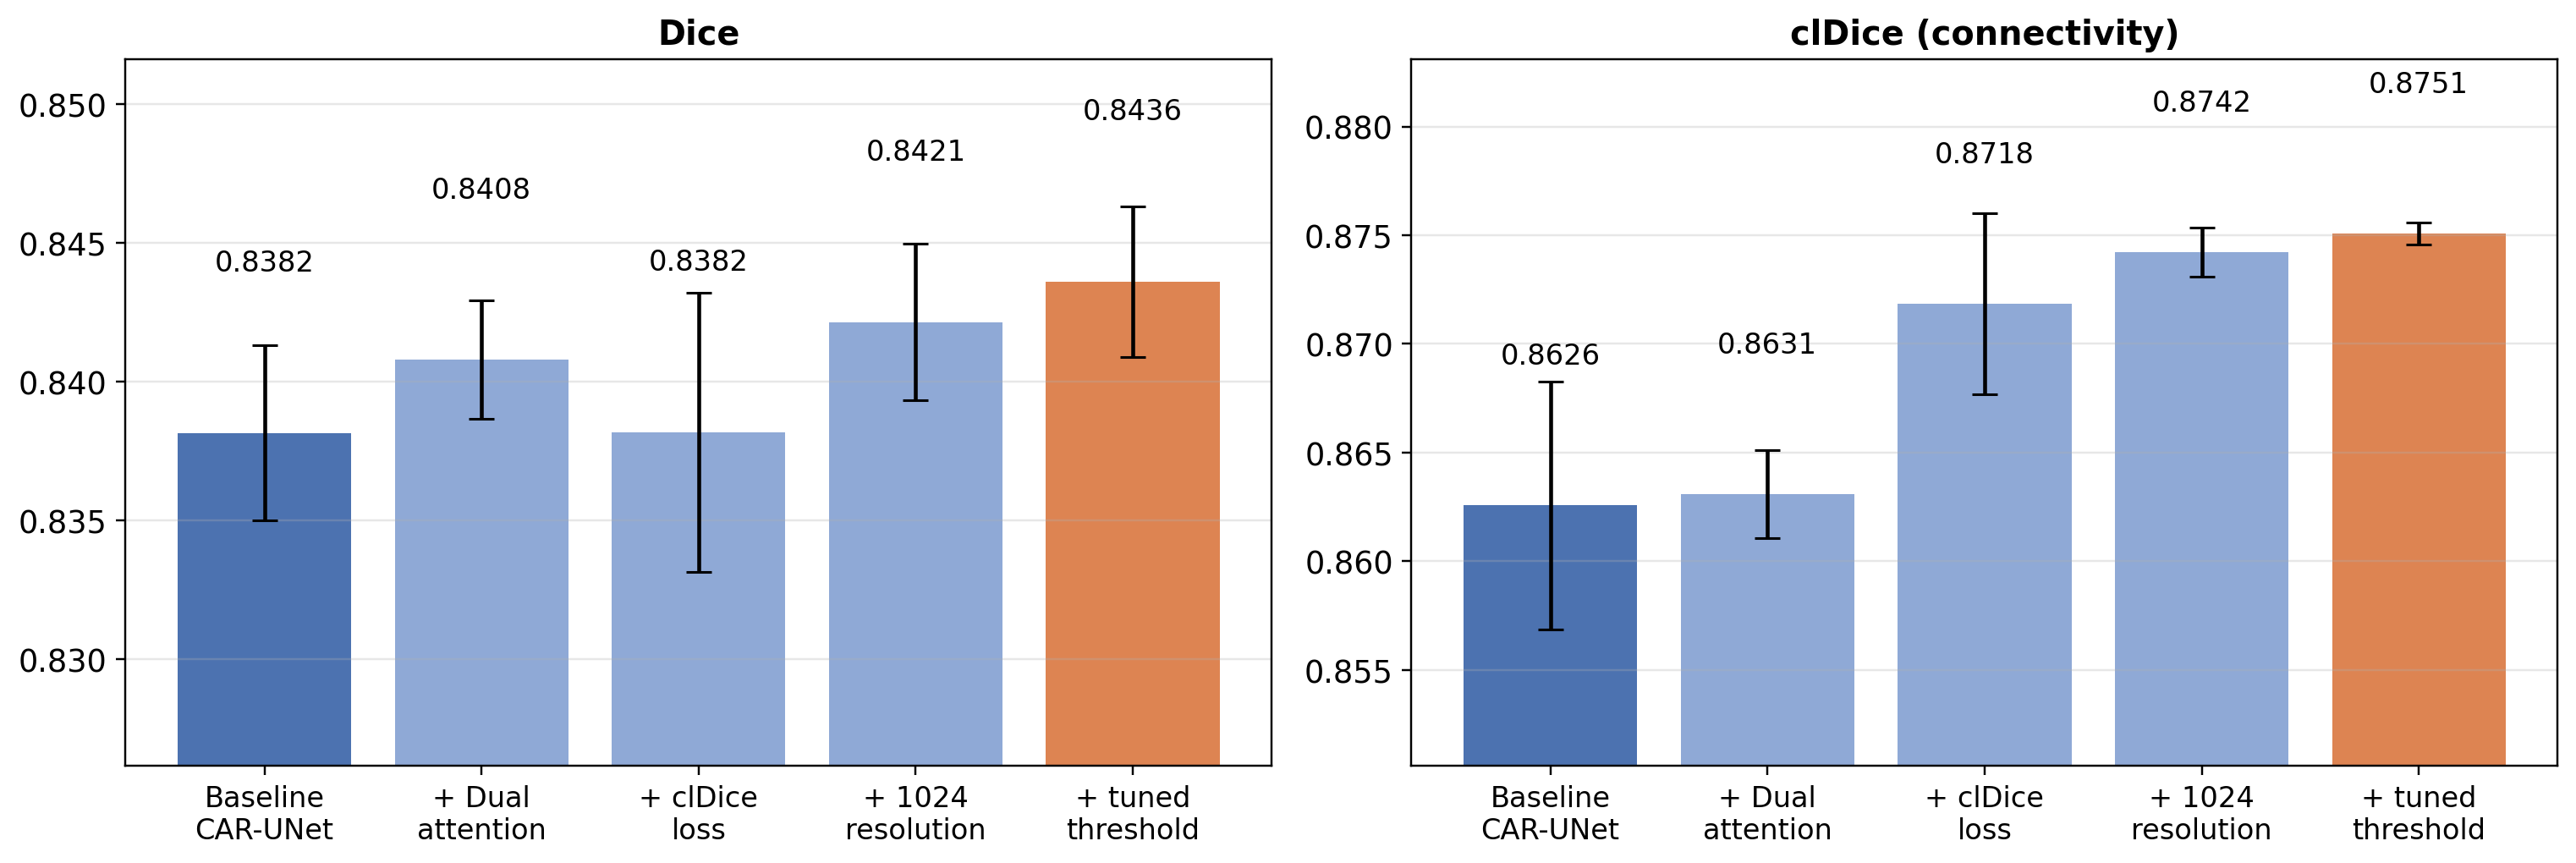
\includegraphics[width=\linewidth]{ablation.png}
    \end{column}
    \begin{column}{0.39\textwidth}
      \scriptsize
      \textbf{Dual attention}: fewer false vessels, most stable.\\
      \textbf{clDice}: big jump in connectivity and sensitivity; Dice flat (more detections at 0.5).\\
      \textbf{1024}: Dice and precision up, thin vessels kept.\\
      \textbf{Threshold}: turns that precision into more vessels found.
    \end{column}
  \end{columns}
\end{frame}

\begin{frame}{Qualitative results: side by side}
  \begin{columns}[c]
    \begin{column}{0.72\textwidth}
      \centering
      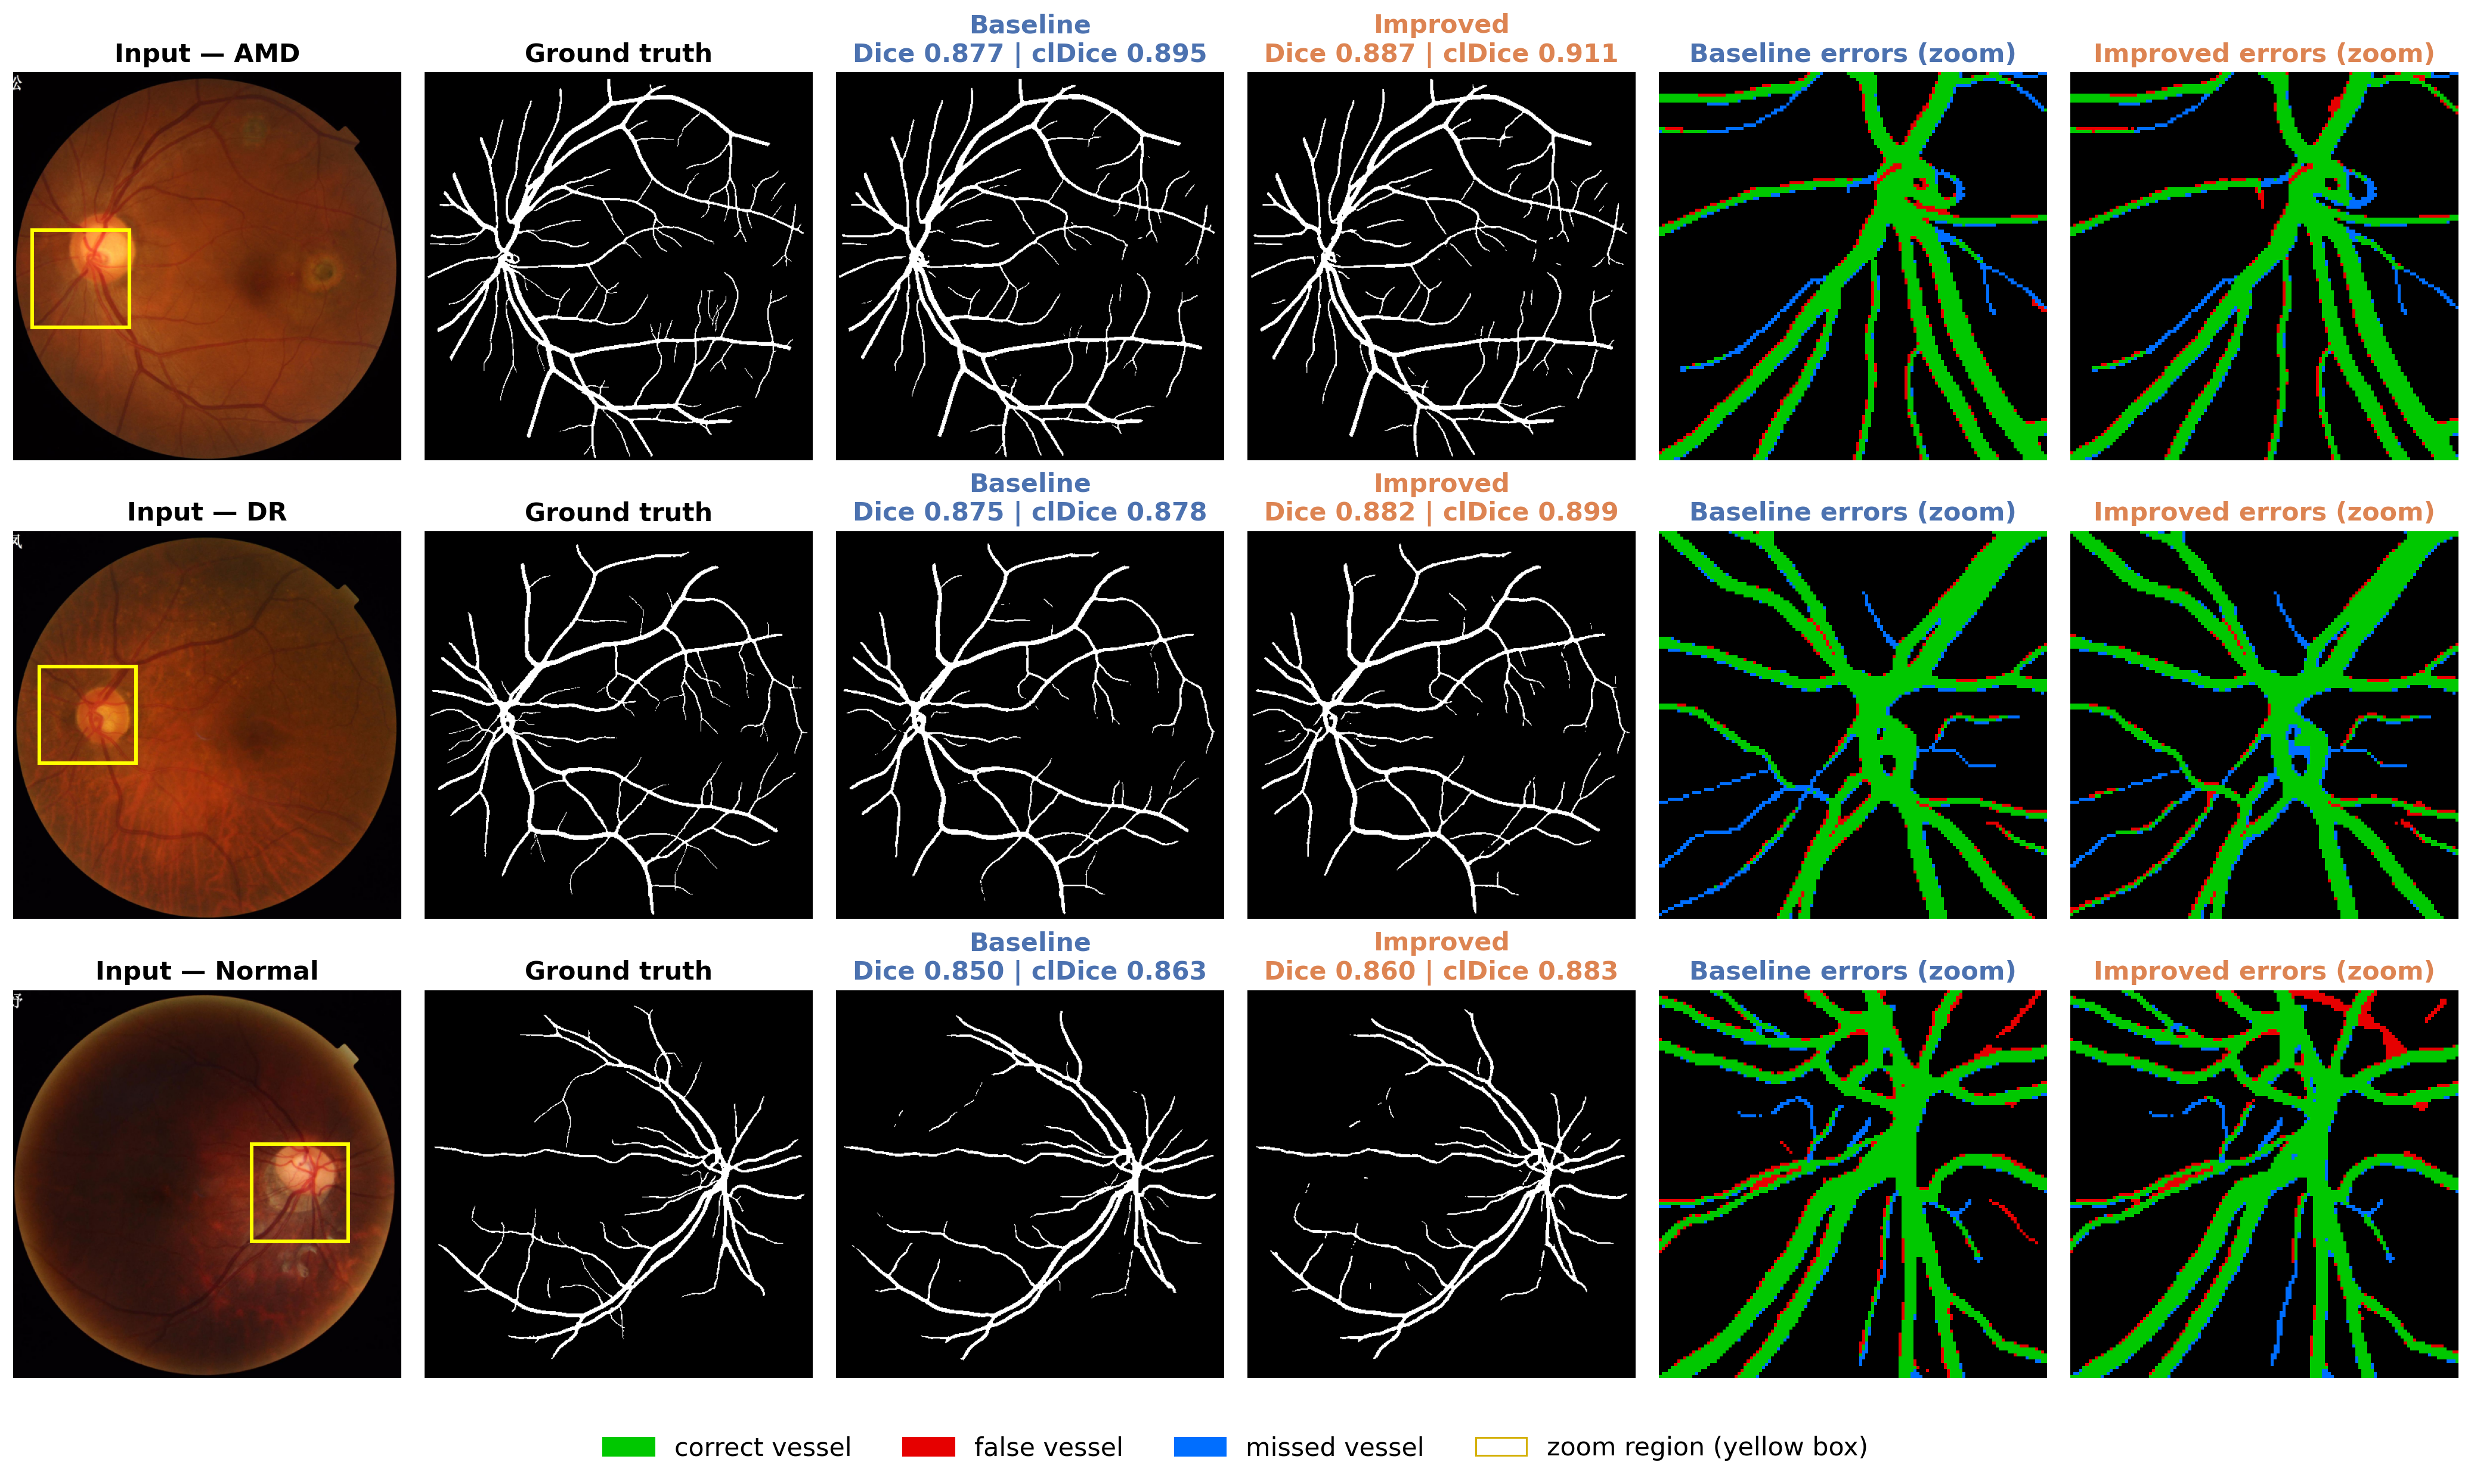
\includegraphics[width=\linewidth]{compare_combined.png}
    \end{column}
    \begin{column}{0.27\textwidth}
      \begin{itemize}\setlength\itemsep{4pt}\scriptsize
        \item Same test images and ground truth; both models run live; median case of each disease (not cherry-picked).
        \item The improved model scores higher on every example (Dice and clDice).
        \item Zoom (yellow box = region with most thin vessels): \textcolor{blue}{\textbf{blue}} = missed, \textcolor{red}{\textbf{red}} = false, \textcolor{good}{\textbf{green}} = correct.
        \item Improved model: \textbf{fewer blue gaps} -- thin branches found and connected; a few extra red pixels (the precision cost).
      \end{itemize}
    \end{column}
  \end{columns}
\end{frame}

\begin{frame}{Analysis: where the gains come from -- and what did not work}
  \begin{columns}[T]
    \begin{column}{0.48\textwidth}
      \begin{table}
        \caption{Dice and clDice per disease (3 seeds).}
        \footnotesize
        \begin{tabular}{@{}lcccc@{}}
          \toprule
          & \multicolumn{2}{c}{Dice} & \multicolumn{2}{c}{clDice} \\
          Disease & Base & Ours & Base & Ours \\
          \midrule
          AMD & 0.8643 & \textbf{0.8671} & 0.8884 & \textbf{0.8978} \\
          DR & 0.8562 & \textbf{0.8585} & 0.8807 & \textbf{0.8895} \\
          Glaucoma & \textbf{0.7958} & 0.7947 & 0.8178 & \textbf{0.8227} \\
          Normal & 0.8363 & \textbf{0.8541} & 0.8635 & \textbf{0.8904} \\
          \bottomrule
        \end{tabular}
      \end{table}
      \footnotesize
      \textbf{Thin vessels:} thin-vessel recall 0.781 $\rightarrow$ 0.788 (139/200 images); Dice against the 1024 ground truth \textbf{0.857 $\rightarrow$ 0.880} (+2.2 points).
    \end{column}
    \begin{column}{0.5\textwidth}
      \textbf{What worked}
      \begin{itemize}\setlength\itemsep{1pt}\footnotesize
        \item Gains concentrate on thin vessels and connectivity -- exactly the target.
        \item Connectivity improves in every disease group; Normal gains most.
      \end{itemize}
      \textbf{What did not work (honest)}
      \begin{itemize}\setlength\itemsep{1pt}\footnotesize
        \item \textbf{Flip TTA} lowered Dice for most models: they segment flipped images up to $\sim$2\% worse, so averaging hurts. Validation now decides when to use it.
        \item \textbf{Glaucoma} is not improved -- low contrast, fewer visible vessels.
        \item Two very poor-quality test images fail for every model (Dice $<$ 0.1).
        \item Precision drops 0.4 points -- the price of finding more vessels.
        \item The 1024 model needs $\sim$1.6$\times$ training time.
      \end{itemize}
    \end{column}
  \end{columns}
\end{frame}

% =============================================================================== CLOSING
\section{Conclusion}

\begin{frame}{Conclusion, future work, contributions and references}
  \begin{columns}[T]
    \begin{column}{0.49\textwidth}
      \textbf{Conclusion}
      \begin{itemize}\setlength\itemsep{1pt}\scriptsize
        \item Replicated CAR-UNet on FIVES under a fair protocol; it beats U-Net, as the paper claims.
        \item Four targeted changes give \textbf{Dice 0.8436}, IoU 0.7379, clDice 0.8751 -- better than the baseline on 9 of 11 metrics, all significant.
        \item Largest gains on thin vessels (+2.2 Dice points at 1024) and connectivity (+1.25).
      \end{itemize}
      \textbf{Future work}
      \begin{itemize}\setlength\itemsep{1pt}\scriptsize
        \item Focus on Glaucoma and low-quality images (FIVES quality labels).
        \item Full 2048$\times$2048 training on a larger GPU.
        \item A lighter model (16 filters, as in the paper) for faster screening.
      \end{itemize}
      \vspace{4pt}
      {\small\textbf{Thank you -- questions welcome.}}
    \end{column}
    \begin{column}{0.49\textwidth}
      \begin{table}
        \caption{Member contributions.}
        \tiny
        \begin{tabular}{@{}p{0.34\linewidth}p{0.60\linewidth}@{}}
          \toprule
          Member & Contribution \\
          \midrule
          Abhishek Karthik J & \fillme{e.g.\ model implementation, training} \\
          \fillme{Member 2} & \fillme{e.g.\ data pipeline, preprocessing} \\
          \fillme{Member 3} & \fillme{e.g.\ evaluation, ablation, figures} \\
          \fillme{Member 4} & \fillme{e.g.\ report, literature review} \\
          \bottomrule
        \end{tabular}
      \end{table}
      \vspace{-6pt}
      \textbf{\small References}\\[-2pt]
      \tiny
      \nocite{*}
      \bibliographystyle{ieeetr}
      \bibliography{refs}
    \end{column}
  \end{columns}
\end{frame}

\end{document}
